%  A simple AAU report template.
%  2015-05-08 v. 1.2.0
%  Copyright 2010-2015 by Jesper Kjær Nielsen <jkn@es.aau.dk>
%
%  This is free software: you can redistribute it and/or modify
%  it under the terms of the GNU General Public License as published by
%  the Free Software Foundation, either version 3 of the License, or
%  (at your option) any later version.
%
%  This is distributed in the hope that it will be useful,
%  but WITHOUT ANY WARRANTY; without even the implied warranty of
%  MERCHANTABILITY or FITNESS FOR A PARTICULAR PURPOSE.  See the
%  GNU General Public License for more details.
%
%  You can find the GNU General Public License at <http://www.gnu.org/licenses/>.
%
\input{setup/preamble.tex}% package inclusion and set up of the document
\input{setup/hyphenations.tex}% 
\input{setup/macros.tex}% my new macros

\begin{document}
%frontmatter
\pagestyle{empty} %disable headers and footers
\pagenumbering{roman} %use roman page numbering in the frontmatter
\input{sections/frontpage.tex}
\input{sections/colophon.tex}
\pdfbookmark[0]{English title page}{label:titlepage_en}
\aautitlepage{%
  \englishprojectinfo{
    Double Tracking Antennas for \\
    UAS Communication %title
  }{%
    Multivariable Control %theme
  }{%
    Spring Semester 2016 %project period
  }{%
    CA832 % project group
  }{%
    %list of group members
    Alvaro Perez Ortega\\ 
    Kenny Lund Lafon\\
    Kelvin Kjærvik Pagels\\
    Robert-Octavian Popescu\\
    Orlando Bastos Vaz
  }{%
    %list of supervisors
    Anders La Cour Harbo
  }{%
    1 % number of printed copies
  }{%
    \today % date of completion
  }%
}{%department and address
  \textbf{Electronics and IT}\\
  Aalborg University\\
  \href{http://www.aau.dk}{http://www.aau.dk}
}{% the abstract
  In an Unamanned Aircraft System (UAS) scenario, one of the main goals is to secure Line-of-Sight (LOS) between the Unmanned Aicraft (UA) and the Ground Station (GS). Moreover, in most cases permanent communication between systems must be assured. Such that, tracking directional antennas in both ends have been considered to have assure this communication. 

  Furthermore, the tracking is done with the help of a DC servomotor which will turn each antenna. Additionally, different controller's have been tested and tunned for this specific application to achieve valuable results. Also, 2D and 3D simulations of the whole system have been made with the servomotor model and controller integrated.  
  
  The scope of the tracking is to achieve satisfactory link budget over long distances. In such a way, large areas can be covered in any application that requires permanent communication between GS and UA. 
}

\cleardoublepage
% {\selectlanguage{danish}
% \pdfbookmark[0]{Danish title page}{label:titlepage_da}
% \aautitlepage{%
%   \danishprojectinfo{
%     Double tracking antennas for drone communication %title
%   }{%
%     Multivariable control %theme
%   }{%
%     Spring 2016 %project period
%   }{%
%     Group: 832 % project group
%   }{%
%     %list of group members
%     Alvaro Perez Ortega\\ 
%     Kenny Lund Lafon\\
%     Kelvin Kjærvik Pagels\\
%     Robert-Octavian Popescu\\
%     Orlando Vaz
%   }{%
%     %list of supervisors
%     Anders La Cour Harbo
%   }{%
%     1 % number of printed copies
%   }{%
%     \today % date of completion
%   }%
% }{%department and address
%   \textbf{Elektronik og IT}\\
%   Aalborg Universitet\\
%   \href{http://www.aau.dk}{http://www.aau.dk}
% }{% the abstract
%   Her er resuméet
% }}
\cleardoublepage
\pdfbookmark[0]{Contents}{label:contents}
\pagestyle{fancy} %enable headers and footers again
\tableofcontents
\listoftodos
\input{sections/preface.tex}
\cleardoublepage
%mainmatter
\pagenumbering{arabic} %use arabic page numbering in the mainmatter

\chapter{Introduction}\label{ch:intro}

The current legislation prevents the use of UAVs out of the line of sight meaning that the users have to see the aircraft when they are piloting it. However, this legislation will be changed, so it will be possible to control these devices without seeing them. A way to keep a connection with the aircraft is to improve the communication systems with the ground station. Hence, this regulation will allow the introduction of UAVs in new fields where they can optimize humans' tasks. For instance, these new UAVs can be used to patrol huge forest areas in order to detect fire starts (aircraft equipped with a thermal camera), instead of having some fire lookout towers preventing this catastrophe. This surveillance, that has to be done day and night in large areas, would not involve risks for human beings and would also be cheaper. 

%This solution that would improve the actual one that is lookout towers and human patrols...%

%PREVIOUS FIRST PARAGRAPH% 
%The current legislation prevents the people to control UAVs out of the line of sight, which means that the users need to see the aircraft when they are piloting it. However, this legislation will change and it will be possible to control this device using a camera and a system which allows the communication between the ground station and the UAV. So, in order to have these mechanisms, it is necessary to solve some issues that, until now, were not studied. The connection between them is one of the main problems because it requires new skills that the old devices don't have. This new legislation allows the introduction of UVAs in new fields where they can perform some functions that the humans are not able to do. For instance, these new UAVs can be used to patrol huge forest areas in order to detect fire starts, instead of having some fire lookout towers that are ineffective against this catastrophe. This surveillance, that has to be done day and night in large areas, would be cheaper without risks for human beings.%

%%%%Currently, the

In this project, the challenge is to maintain the connection between the UAV and the ground station, not only when the distance is a few meters, but also when it is tens of kilometers. Such a zone can include mountainous areas, which are physical barriers, flat areas and zones where the atmosferic conditions can be a problem for the navigation (for example, windy or rainy places). Due to the difficulty or, sometimes, the impossibility of exceed these obstacles, it is mandatory to improve the connection to decrease their effect. In other words, the aircraft needs to be prepared for this barriers in order to have a reliable communication with its ground station. 

Thus, the main goal of this project is to increase the distance between the devices using two tracking antennas (one on the ground and one on the aircraft) that are able to keep the communication. Directional antennas can solve this problem  because it is possible to use their main lobes to guarantee a reliable connection. As a result, it will be necessary to develop a system capable of controlling both antennas to make them point at each other.

%PREVIOUS THIRD PARAGRAPH%
%In this project, the challenge is to maintain the connection between the UAV and the ground station when the distance that separates them is some tens of kimometers. This huge distance involves not only flat areas, but also mountainous areas which are physical barriers that don’t allow a correct communication and where the atmospheric conditions can be really hard (for example, windy or rainy places). However, the aircraft needs to be prepared structurally for a set of conditions in which the communication between the ground station and the UAV is reliable. The signal emitted and received by both antennas needs to be strong enough to overtake every obstacle. Thus, the main goal of this project is to communicate with a UAV through two tracking antennas (one on the ground and one on the other on the aircraft) when the distance between them is too big. In order to improve the communication it will be necessary to explore the best qualities of the antennas. In other words, directional antennas will be the best choice because it is possible to use their main lobes to guarantee a reliable connection. So that, it will be necessary to develop a system able to control both antennas to put them pointing at each other.%


Before the new legislation, due to the fact that the UAV was flying close to the ground station, the signal was strong enough to maintain the contact. For example, omnidirectional antennas are able to do this task although they don't have any prime direction. On the other hand, when the distance between the aircraft and the ground station increases, the contact becomes difficult because the loss of signal increases a lot. The limited frequency and bandwidth by means of law and the limitated antenna power and size are other constraints that can compromise the detection of the signal. 


%Our case: limited frequency and bandwidth by means of the Law. the can't emit a signal.......(read more about this)
%Limited antenna power and size. The power of the antennas is not infinite so it is difficult to make sure that the signal will be received by the receiver. The mountains are physical barriers because the signal can't pass through it - the drone needs to fly in a high altitude
%The weather degradates the signal and it will be difficult to communicate through certain conditions. The only solution is to try to point the antennas to each other because it will increase the probability of communication.
%Controller used controls 2 angles of both antennas (just say that not explain anything).

%\chapter{Scenario}\label{ch:scenario}

\section{Communication}


The free space path loss (FSPL) is the loss in signal strength that occurs when an electromagnetic wave travels over a line of sight path in free space. In these circumstances there are no obstacles that might cause the signal to be reflected, refracted, or that might cause additional attenuation. Equation \ref{eq:path_losses} represents the loss in signal strength.

\begin{equation}\label{eq:path_losses}
L = 20log\left (\frac{4\pi d}{\lambda} \right)
\end{equation}

The wave length can also be described by a relationship between the frequency and the velocity which is the light speed because radio waves are electromagnetic waves. This relationship is described by the equation \ref{eq:vel_freq_wavelen1}.

\begin{equation}\label{eq:vel_freq_wavelen1}
\lambda = \frac{c}{f}
\end{equation}

Considering an area of a 

\begin{equation}\label{eq:vel_freq_wavelen2}
\lambda = \frac{c}{f} = \frac{3\times 10^{8}}{f\times 10^{6}}=\frac{300}{f}=\frac{3}{10f}
\end{equation}

\section{Rescue missions}
\subsection{What do they do today?}
\subsection{Compare the rescue missions}

\section{Pipeline survey}
The pipeline survey could be to transport oil from a factory to another facility. To ensure that there is no thiefs that want to steal the oil, they have to hire people to patrol. Instead they could use a drone to search the area.
\begin{figure}[hb]
  \centering
 % 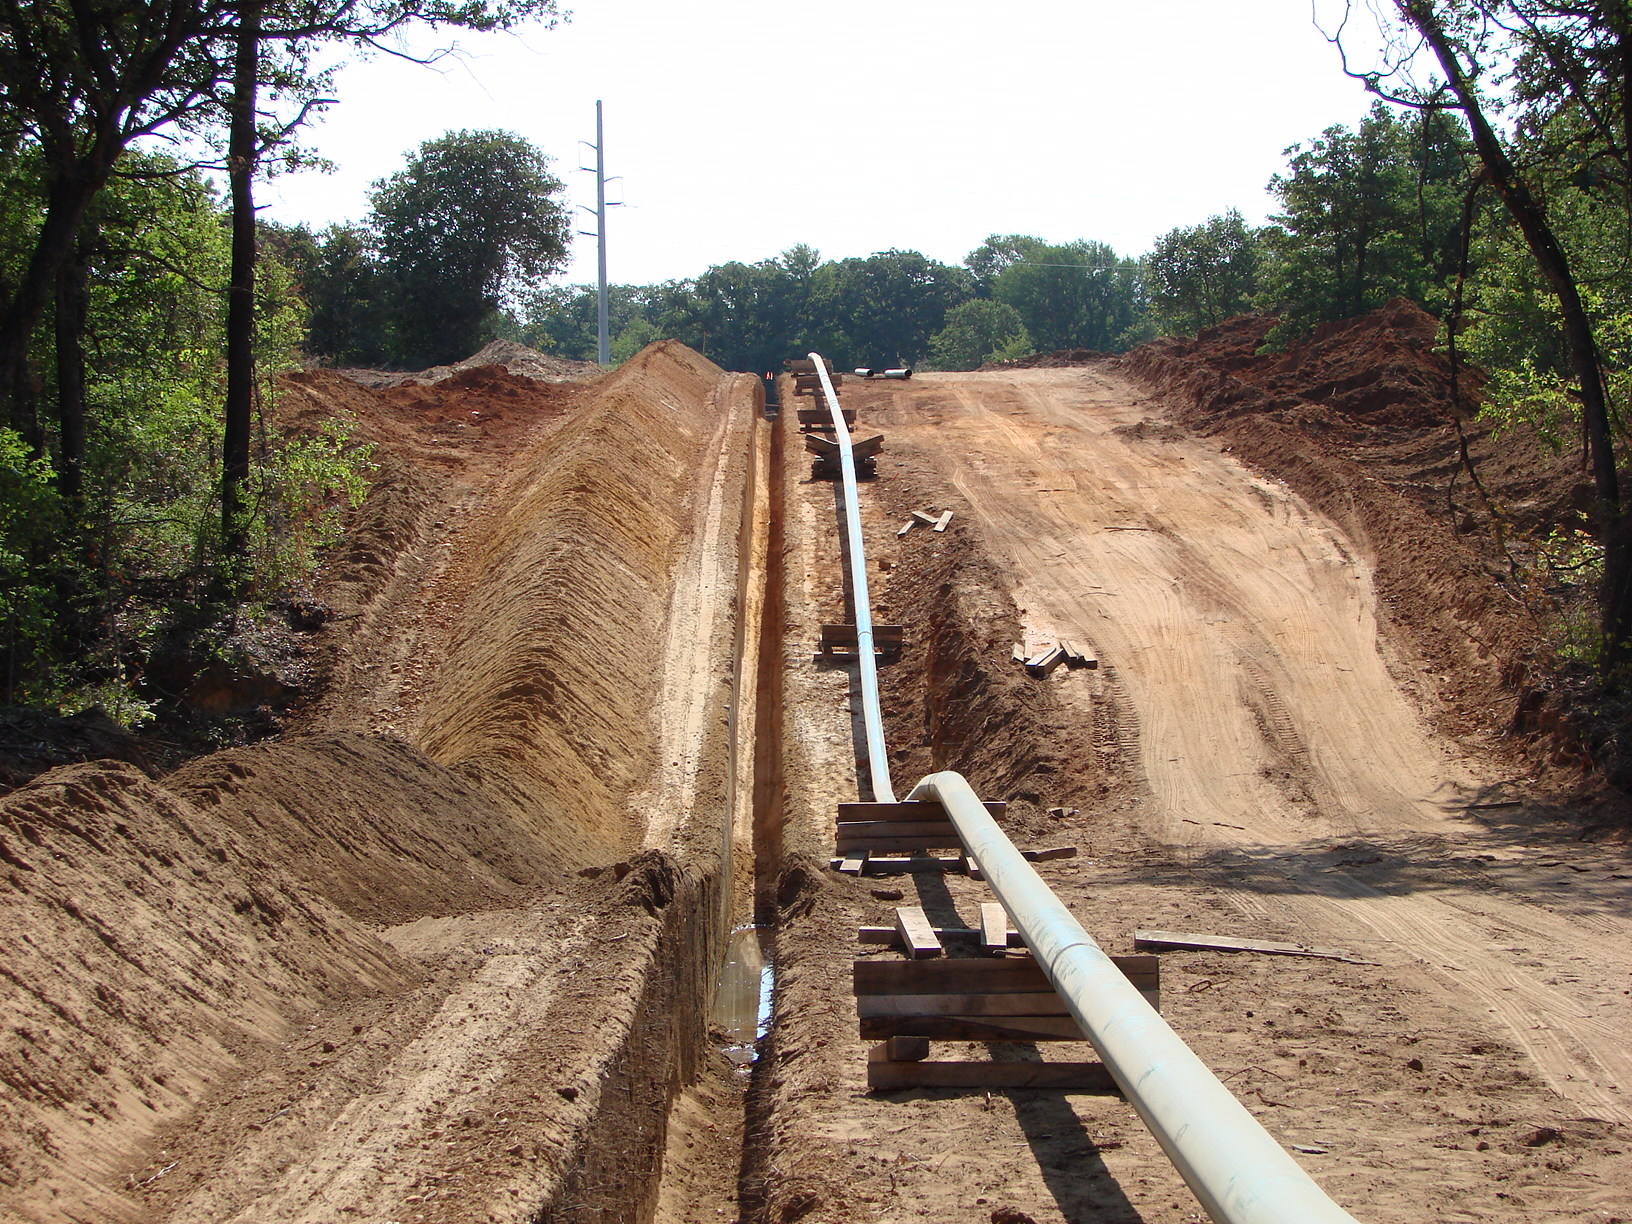
\includegraphics[width=3in]{figures/pipelinesurvey.png}
  \caption[Pipeline survey]
   {Pipeline survey}
\end{figure}
Potential danger
\begin{itemize}
\item Terrorist
\item Thiefs
\end{itemize}

\chapter{Unmanned Aerial System Overview}\label{ch:uas}

The main goal of this project is to try to increase the distance between the aircraft and the ground station using two tracking antennas. However, the increase of the distance will reduce the quality of the signal that is received and sent by both antennas. In order to keep the communication, it is essential to have the proper physical infrastuctures to be able to detect both strong and weak signals. These infrastuctures constitute the hardware and they cover every element connected with the vehicle, in the air, and the ground station, on the ground. The previous description of the system as a whole constitutes the Unmanned Aerial System, UAS.

The UAS illustrated in Figure \ref{fig:uas} can be decomposed in the following elements:
\begin{itemize}
	\item Unmanned Aerial Vehicle, UAV
	\item Ground Station, GS
	\item Antennas
	\item Survey camera
\end{itemize}

\begin{figure}[H]
	\centering
	\includegraphics[scale=0.33]{figures/uas.png}
	\caption{Unmanned Aerial System}
	\label{fig:uas}
\end{figure}

%In order to have some bounds of the system we can have a look at the drone performances:
%\begin{itemize}
%	\item 50 km/h - stability at high speeds 
%	\item 40 minutes - battery autonomy (30 minutes with payload)
%	\item 2400 m - maximum flight altitude (higher if take off from mountain site)
%	\item 50 km - maximum radio communication (with directional antennas)
%	\item under 1 m - absolute positioning of X-Y GPS
%	\item GPS return-to Home (automatically activates when radio link is lost)
%\end{itemize}



\section{Unmanned Aerial Vehicle}\label{sec:drone}

The unmanned aerial vehicle, UAV, commonly called drone, is an aircraft which doesn't need to be piloted by a person inside of the vehicle. Thus, it is necessary a system which is able to control the UAV in order to accomplish the desired task. This system gives parcial or total automony to the aircraft, which means that it can be, respectively, a remote control from an operator or onboard computers, which are prepared to act depending on the situation with which the drone is dealing. The remote control from an operator can be either on the ground, in a GS, either in the air, in another vehicles.

Nowadays, the use of UAVs is increasing due to the huge number of tasks that these vehicles can perform. Surveying, mapping, aerial photography, monitoring and militar applications are some examples of tasks that are executed by these aircrafts.  

In this project, the operator will be on the ground and, therefore, the UAV will be controlled by a couple of tracking antennas. One antenna will be on board and the other will be on the ground in a base station which will receive and send information from and to the aircraft. 

For this project it will be used, as an example, the eBee that can be observed in Figure \ref{fig:ebee}. This aircraft was developed by a company called senseFly and has three different models: eBee, the mapping drone, eBee RTK, the survey-grade mapping drone, eBee Ag, the precision agriculture drone. Each model was created for a specific task, however the main caracteristics are common to every model. The shape of these aircrafts is the same as the airplane ones, the weight varies between 0.69 Kg and 0.73 Kg, the wingspan is 96 cm and they are made of EPP foam and carbon. They are equipped with a 11,1 V baterry, which allows a flight time between 40 and 50 minutes, and with a WX camera (18.2 MP) which can be changed by another cameras like the thermoMAP. The thermoMAP captures thermal videos and still images which allows the creation of a full thermal map of a site. The Ground Sampling Distance (GSD), that is the distance measured on the ground between the center of two consecutive pixels when the picture was taken from the air, varies between 1.5 cm and 2 cm (maximum values). 
 
\begin{figure}[H]
  \centering
  \includegraphics[scale=0.45]{figures/eBee.png}
  \caption[The professional mapping drone eBee]
   {The professional mapping drone \textit{eBee} \href{https://www.sensefly.com/drones/ebee.html}{(www.sensefly.com)}. Fully autonomous drone to capture high-resolution aerial photos that can transform into accurate 2D orthomosaics \& 3D models.}
   \label{fig:ebee}
\end{figure}

The accuracy related to the position depends on the existance of ground control points (GCP). In the table \ref{accuracy} it is described the vertical and horizontal accuracy for each model.

\begin{table}[h!]
	\centering
	\begin{tabular}{|c||c|c|c|}
		\hline
		Parameter & eBee & eBee RTK & eBee Ag\\ \hline\hline
		Horizontal Accuracy (with GCPs) & Down to 3 cm & - & Down to 4 cm\\ \hline
		Vertical Accuracy (with GCPs) & Down to 5 cm & - & Down to 7 cm\\ \hline
		Horizontal Accuracy (without GCPs) & 1-5 m & Down to 3 cm & 1-5 m\\ \hline
		Vertical Accuracy (without GCPs) & 1-5 m & Down to 5 cm & 1-5 m\\ \hline
	\end{tabular}
	\caption{Table of horizontal and vertical accuracy of the eBee models}
	\label{accuracy}
\end{table}

The software that is responsible for controlling and planning the flight is called eMotion. This is a ground station software and is supplied with every eBee model.
\section{Ground Station}\label{sec:gs}


			! !	! ! ! ! ! ! ! ! ! ! ! !
! ! ! ! ! ! ! WE NEED SOMETHING HERE ! ! ! ! ! !
			! ! ! ! ! ! ! ! ! ! ! ! ! !
\section{Antennas}\label{sec:antennas}

As it was mentioned before the often approach to this kind of communication is to use directional antennas.
The reason to do this, is that a directional antennas are known for having a very high gain in a narrow beam width, whereas on the other hand, an omnidirectional antenna has a lower gain while having a very broad beam width \cite{Collin85}.
Therefore, the use of this first type of antennas will allow us to improve the quality of the radio link as long as the antennas are pointing at each other.

The antennas used for the GS and the UA are different by means of weight and size. The preference of using them is based on the application at hand, thus for:
\begin{itemize}
	\item GS - Parabolic (grid) directional antenna 
	\item UA - Patch directional antenna
\end{itemize}

A parabolic antenna in an antenna that uses a parabolic reflector and a curved surface to direct the radio waves and its main advantage is that it has a high directivity. This type of antennas are able to produce a narrow beam width which allow them to have some of the highest gains. Parabolic antennas, due to their high gain, are intensively used for carry telephone and television signals between nearby cities \cite{Collin85}\cite{parabolic}.

Patch antenna, which is the original type of microstrip, is a low profile antenna that can be mounted on a flat surface and it consists in a rectangular sheet of metal. These antennas are very useful because they are very thin and they provide a quite high directivity \cite{Collin85}\cite{patch}.

Later on, in Chapter \ref{ch:model} a modelling process to simulate these types of directional antennas will be addressed.
\section{DC Servomotor}\label{sec:servo_motor}

The control of both antennas requires the use of four motors which will be able to change its orientation (two motors per antenna in order to control two different angles). In this project, the DC servomotor was chosen because it can be either a rotary or a linear actuator which allows a precise control of angular or linear position, velocity and acceleration.

The servomotor can be described in two different parts: an electrical motor and a servomechanism. The electrical motor is a DC motor which is able to convert electrical power into rotational mechanical power and the servomechanism is the group of elements connected with the DC motor. The shaft of the DC motor is coupled with another shaft denominated output shaft. The connection is made through a gear assembly which is not only responsible for the connection between both shafts, but also for the reduction of the RPM of the motor’s shaft (figure \ref{servomotor_expl1}).

\begin{figure}[H]
\centering
\includegraphics[scale=0.7]{figures/servomotor_expl1.png}
\caption{Connection between the output shaft and the DC motor}
\label{servomotor_expl1}
\end{figure}

The output shaft is also connected with a potentiometer by another gear assembly and, during its rotation, the knob rotates and creates an electrical signal. This signal increases proportionally with the angular movement of the potentiometer knob. The connection between the output shaft and the potentiometer can be
observed in the figure \ref{servomotor_expl2}.

\begin{figure}[H]
\centering
\includegraphics[scale=0.61]{figures/servomotor_expl2.png}
\caption{Connection between the output shaft and the potentiometer}
\label{servomotor_expl2}
\end{figure}

The previous described gears are involved in the gear mechanism which is responsible for the transformation of the original input speed provided by the DC motor into a slower output speed which is practical and widely applicable. 

The potentiometer is also connected with an error detector feedback amplifier where the electrical potential (from the potentiometer) and the input command voltage (the signal that represents the desired angle) are compared. The output of the error detector amplifier is called electrical input of the DC motor and is represented in the figure \ref{servomotor_expl3}. When the electrical potential equals the input voltage, which means that the shaft is in the desired position, the input of the DC motor becomes zero and the motor stops rotating until the next command.

\begin{figure}[H]
\centerline{
\includegraphics[scale=0.6]{figures/servomotor_expl3new.png}}
\caption{Servomotor’s feedback}
\label{servomotor_expl3}
\end{figure}

In order to be able to do the procedure described in the figure \ref{servomotor_expl3} it is necessary to apply a restricted input voltage signal in regular intervals. Servomotors operate from 4.8V to a 6V supply voltage, but 5V is the typical value. 

On the other hand, the pulse should have a specific width (PWM – Pulse Width Modulation) because it will be responsible for the amount of rotation. Typically, the duration of the pulse varies from 1ms to 2.2ms and the frequency from 50Hz to 60Hz. The size of the pulse will result in a lesser or greater rotation. The figure \ref{signal_servo} is an example of the relation pulse-rotation and describes three different cases. For instance, if the duration of the pulse is 1.25ms, the servomotor will rotate 90 degrees.

\begin{figure}[H]
\centering
\includegraphics[scale=0.5]{figures/signal_servo.jpg}
\caption{Examples of the relation between the PWM and the rotation}
\label{signal_servo}
\end{figure}

Based on the previous explanation, the servomotor requires a power supply unit and the information about the rotation that should be done through an electrical signal. Hence, this motor needs three different terminals (the figure \ref{cable_servo} is one example of the terminals of a servo motor):
\begin{itemize}  
        \item Orange - Position signal (PWM pulses).
        \item Brown - $V_{cc}$ (from the power supply unit). 
        \item Red - Ground.
\end{itemize}

\begin{figure}[H]
\centering
\includegraphics[scale=0.5]{figures/cable_servo.png}
\caption{Servo motor with its three different terminals}
\label{cable_servo}
\end{figure}



\subsection{Frames}

\begin{frame}{Frames}{}

  \begin{itemize}
  \item Geodetic Coordinate System
  \item Earth-Centered Earth-Fixed (ECEF)
  \item North-East-Down (NED)
  \item Body Coordinate System
  
  \end{itemize}

 

  
\begin{figure}[H]
\centerline{
\includegraphics[scale=0.35]{figures/GeoTemp1.png}}
\label{fig:frames}
\end{figure}  
  
  
\end{frame}


\section{Geodetic Coordinate System}\label{sec:coord}

\begin{figure}[H]
   \centering
    \includegraphics[width=.70\textwidth]{figures/GeoTemp1.png} 
    \label{fig:Geodetic}
    \caption{Geodetic, ECEF and local NED Frames.}  
\end{figure}

\paragraph{}The geodetic coordinate system is widely used in GPS-based navigation. Note that it is not an usual Cartesian coordinate system but a system that
characterizes a coordinate point near the earth’s surface in terms of longitude, latitude, and altitude (or height), which are respectively denoted by $\lambda$, $\varphi$, and h (yellow lines) in figure \ref{fig:Geodetic}.

\paragraph{}The \textit{World Geodetic System} is a standard used in cartography, geodesy and navigation. This standard sets reference points based on an ellipsoidal model of the earth and a gravitational equipotential surface that defines the nominal sea level. Its latest version is \textbf{WGS84}, and that is the one used throughout this project. 

The longitude measures the rotational angle (ranging from $-180$ to $180$ degrees) between the Prime Meridian and the measured point. The latitude measures the angle (ranging from $-90$ to $90$ degrees) between the equatorial plane and the normal of the reference ellipsoid that passes through the measured point. The height (or altitude) is the local vertical distance between the measured point and the reference ellipsoid.


\section{Earth-Centered Earth-Fixed (ECEF) Coordinate System}\label{sec:ecef}

\paragraph{}The Earth-Centered Earth-Fixed (ECEF) is a cartesian system which rotates with the Earth around its spin axis (blue lines in Figure \ref{fig:Geodetic1}), assigning a fixed set of coordinates for a specific point on the Earth's surface. The origin and axis of this system are defined as follows:
\begin{itemize}
\item{The origin (\textbf{$O_{e}$}) is located at the center of mass of the Earth. Hence the so-called s"Earth-Centered".}
\item{The Z-axis (\textbf{$Z_{e}$})} is set along the International Reference Pole (IRP).
\item{The X-axis (\textbf{$X_{e}$})} is set along the International Reference Meridian (IRM), intersecting the sphere (or elipsoid) of the Earth at 0$^{\circ}$ latitude (Equator) and 0$^{\circ}$ longitude (Greenwich).
\item{The Y-axis (\textbf{$Y_{e}$})} is orthogonal to both the Z and X axis described before by the usual right-hand rule.
\end{itemize}

\paragraph{}Even though ECEF coordinate frame is not commonly chosen as the final form to express the coordinates, it is frequently used as an intermediate step to convert between the \textbf{WGS84} geodetic system to the North-East-Down (NED) coordinate system as it will be shown later on.
\section{North-East-Down (NED) Coordinate System}\label{sec:ned}

\paragraph{} The North-East-Down is a geographical coordinate system fixed to the Earth's surface, and, precisely because of this, is also known as \textbf{local tangent plane (LTP)} or ground coordinate system (green lines in Figure \ref{fig:Geodetic1}). The origin and axis of this system are defined as follows: 
\begin{itemize}
\item{The origin (\textbf{$O_{n}$}) is located at a arbitrary point on the Earth's surface.}
\item{The X-axis (\textbf{$X_{n}$}) points towards the geodetic north.}
\item{The Y-axis (\textbf{$Y_{n}$}) points towards the geodetic east.}
\item{The Z-axis (\textbf{$Z_{n}$}) points downward along the ellipsoidal normal, set by the right-hand rule.}
\end{itemize}

\paragraph{} The local NED frame plays a very important role in flight control and navigation.
Navigation of small-scale UAs is normally carried out within this frame. It will later be shown that during this work 2 different local NED frames would be described. One being with the origin fixed at the Ground Station location and one with an origin at the center of gravity of the UA at all times. This is the so-called \textbf{Vehicle-carried NED}, represented with the \textit{nv} subscript in Figure \ref{fig:NED1}\cite{Houghton70}.\\
Note that, strictly speaking, the axis of the Vehicle-carried NED are not completely aligned with the ones of the local NED , varying due to the movement of the vessel. However, for smalls aircrafts the directional difference is completely negligible. Furthermore, $h = -z$ is often used to denote the actual height of the UA.

\paragraph{} Now, to define a point within this local frame, spherical coordinates will be used. In mathematics, a spherical coordinate system is a coordinate system for three-dimensional space where the position of a point is specified by three numbers: the \textbf{radial distance} of that point from a fixed origin ($\rho$), its \textbf{polar angle} measured from a fixed zenith direction ($\theta$), and the \textbf{elevation angle} of its orthogonal projection on a reference plane, measured from a fixed reference direction on that plane ($\phi$).\\
The way these spherical coordinates are defined during this specific project are shown in Figure \ref{fig:Spherical1}.
\begin{figure}[H]
   \centering
    \includestandalone[width=.60\textwidth]{figures/3D_Sphcoord} 
    \caption{Spherical Coordinates in NED Frame.}
    \label{fig:Spherical1}
\end{figure}

\paragraph{} Note how this cartesian coordinate system is defined such that $\theta = 0$ is aligned with the east ($y$) axis of the NED frame and  $\phi > 0$ is defined for negative values or $z$, i.e., positive height on the surface of the Earth.
Additionally, it is necessary to define a unique set of spherical coordinates for each point, and therefore restricting the range of these parameters is required. In our case the coordinates will be limited as follows:
\begin{align*}
& \rho \geq 0 \\
& -\pi \leq \theta < \pi \\
& \frac{-\pi}{2} \leq \phi \leq \frac{\pi}{2}
\label{eq:los_distToHorizon}
\end{align*}
These constraints define the conversion between Cartesian and Spherical coordinates such that:
\begin{align*}
x &=  \rho\cos\phi\sin\theta  & \rho &= \sqrt{x^{2} + y^{2} + z^{2}} \\
y &= \rho\cos\phi\cos\theta   & \theta &= \arctan\left(x\right)\\
z &= \rho\sin\phi       & \phi &=  \arctan\left(-z\right)
\label{eq:los_distToHorizon}
\end{align*} 


\section{Body Coordinate System}\label{sec:body}
This frame has also the origin in the center of gravity of the UAV, however, unlike the vehicle-carried NED, the axis rotate with the craft:
\begin{itemize}
\item{The origin (\textbf{$O_{b}$}) is located at the center of gravity of the UAV.}
\item{The X-axis (\textbf{$X_{b}$}) points in the forward direction.}
\item{The Y-axis (\textbf{$Y_{b}$}) points towards starboard, the right side of the UAV.}
\item{The Z-axis (\textbf{$Z_{b}$}) points downward, set by the right-hand rule.}
\end{itemize}
\begin{figure}[H]
   \centering
    \includegraphics[width=.70\textwidth]{figures/NEDtemp1.png} 
    \caption{Body, vehicle-carried and local NED Frames.}  
    \label{fig:NED1}
\end{figure}

\section{Transformations}\label{sec:body}

\subsection*{From NED to Body}
\paragraph{} The orientation of a Cartesian coordinate system with respect to another can be described in three successive Euler rotations, usually performed about each of the three cartesian axes consequently. During this work we will mainly focus on the transformation between the vehicle-carried NED and the body frame. In order to do this we will follow a specific rotation sequence, moving the reference frame to the referred frame by a Z-Y-X (also called 3-2-1) sequence. These three Euler angles are also known respectively as \textbf{yaw}($\psi$), \textbf{pitch}($\xi$) and \textbf{roll}($\gamma$).

\paragraph{} This way, the transformation from the vehicle-carried NED frame to the Body frame is given by:
\begin{align}
\textbf{P}_{b} = \textbf{R}_{b/nv}\textbf{P}_{nv}
\end{align}
where \textbf{R}$_{b/nv}$ is the \textbf{Rotation matrix}:
\begin{align*}
\textbf{R}_{b/nv} =
\begin{bmatrix}
\cos(\xi)\cos(\psi) & \cos(\xi)\sin(\psi) & -\sin(\xi)\\
\sin(\gamma)\sin(\xi)\cos(\psi) - \cos(\gamma)\sin(\psi) & \sin(\gamma)\sin(\xi)\sin(\psi) + \cos(\gamma)\cos(\psi) & \sin(\gamma)\cos(\xi)\\
\cos\gamma)\sin(\xi)\cos(\psi) + \sin(\gamma)\sin(\psi) & \cos(\gamma)\sin(\xi)\sin(\psi) - \sin(\gamma)\cos(\psi) & \cos(\gamma)\cos(\xi)
\end{bmatrix}
\end{align*}

\paragraph{} However, even though the local NED cordinates is what is necesary to transform to the Body frame, the primary resource that we will have is the GPS position measurements of each of our devices (Ground station and UAV). Therefore a transformation from Geodetic Coordinate Frame to local NED frame is in due. The ECEF Coordinate Frame will be used as an intermediate step during this process.

\subsection*{From Geodetic to ECEF}
Being \textbf{P}$_{g}$ the position of a point in the geodetic system such that is defined by its latitude, longitude and height:
\begin{align}
\textbf{P}_{g} = 
\begin{bmatrix}
\lambda \\
\varphi\\
h
\end{bmatrix}
\end{align}
By using the parameters set by the \textbf{WGS84} standard in section \ref{sec:coord} the tranformed point, \textbf{P}$_{e}$ will be given by
\begin{align}
\textbf{P}_{e} = 
\begin{bmatrix}
\lambda \\
\varphi\\
h
\end{bmatrix}
=
\begin{bmatrix}
(N_{E}+h)\cos(\varphi)\cos(\lambda) \\
(N_{E}+h)\cos(\varphi)\sin(\lambda) \\
(N_{E}(1-\textbf{e}^2)+h)\sin(\varphi)
\end{bmatrix}
\end{align}

\subsection*{From ECEF to NED}
Analogusly to the former transformation, we have
\begin{align}
\textbf{P}_{n} = \textbf{R}_{n/e}\left(\textbf{P}_{e} - \textbf{P}_{e,ref}\right)
\end{align}
where \textbf{P}$_{e,ref}$ is the position of the origin of the local NED frame in ECEF frame and \textbf{R}$_{n/e}$ is the \textbf{Rotation matrix} given by: 
\begin{align*}
\textbf{R}_{n/e} =
\begin{bmatrix}
-\sin(\varphi_{ref})\cos(\lambda_{ref}) & -\sin(\varphi_{ref})\sin(\lambda_{ref}) & \cos(\varphi_{ref})\\
-\sin(\lambda_{ref}) & \cos(\lambda_{ref}) & 0\\
-\cos(\varphi_{ref})\cos(\lambda_{ref}) & -\cos(\varphi_{ref})\sin(\lambda_{ref}) & -\sin(\varphi_{ref})\\
\end{bmatrix}
\end{align*}
where $\varphi_{ref}$ and $\lambda_{ref}$ are the latitude and longitude of the reference point in Geodetic frame.

\chapter{Telecommunication}\label{ch:telecommunication}

Drone communication links are generally either radio frequency (RF) or lasercom (optical). Even though both types currently suffer from bandwidth limitations, lasercom could surpass RF in terms of airborne data transfer rate. However, RF will continue to dominate at the lower altitudes for some time into the future because of its better all-weather capability. Additionally, RF links have the advantage of being much more efficient and usually much less complex than lasercom links.
Data rates for RF links have traditionally been restricted due to limited spectrum and
minimization of communication system size, weight, and power.

Radio waves are a form of electromagnetic radiation with frequencies ranging from 3 kHz to 300 GHz. The size and profile constraints of small drones cannot facilitate communication links on the low-frequency (large wavelength) end of the spectrum. 
On the other hand, atmospheric attenuation as well as attenuation by rain, both
exponential in character, becomes a serious limiting factor to the link distance in
the millimeter wavelength region (>300MHz). 
	
Due to these limitations, small drone communication links are restricted to the very high frequency (VHF), the ultrahigh frequency (UHF), and rarely the super-high frequency (SHF) bands.

\section{Telemetry}
One of the main goal of drone surveillance is to procure relevant data. This is done by means of telemetry which is an automated communication process. In this process the data collected is transmitted to a receiving equipment for further processing and monitoring. 

!!! ADD MORE INFO !!!

!!! ADD FIGURE !!!

!!! HOW WE USE IT ? !!!

\section{MAVLink protocol}
When speaking of digital communication it is required to have a certain communication protocol. Given the fact that, this project deals with drones, a special protocol, namely Micro Air Vehicle Link (MAVLink) has been taken into consideration. This protocol is used in a GNS and drones scenario, where inter-communication between systems is needed in order to transmit GPS location, heading angle and speed.  

\subsection{Packet structure}
For further understanding the packet structure of such a protocol is needed as seen in Table \ref{tab:mavlink}.

\begin{table}[h]
	\centering
	\begin{tabular}{|c||c|c|}
		\hline
		Field name       & Index (Bytes)  & Purpose											     \\ \hline\hline
		Start-of-frame   &      0         & Start of frame transmission 							   \\ \hline
		Pay-load-length  &      1         & Length of payload (n)       							   \\ \hline
		Packet sequence  &      2    	  & Sent sequence counter (detect packet loss)                 \\ \hline
		System ID        & 		3		  & Sending system identification 							   \\ \hline
		Component ID     & 		4 		  & Sending component identification 						   \\ \hline
		Message ID       & 		5 		  & Message identification (correctly decoded)      		   \\ \hline
		Payload          &   6 to (n+6)   & Data into the message, depends on Message ID        	   \\ \hline
		CRC              & (n+7) to (n+8) & Check-sum of packet (excluding packet start sign)          \\ \hline
	\end{tabular}
	\caption{MAVLink packet structure}
	\label{tab:mavlink}
\end{table}

The CRC field ensures message integrity of each packet. Another function of the CRC is to establish that both sender and receiver agree on the message transfer. Additionally, a seed value is appended at the end of the data when computing the CRC, generated with every new message.

\subsection{Messages}
As stated above the payload from the packets are MAVLink messages. Also, every message can be identified by its ID field on the packet. Additionally, an XML document (in MAVLink source) has the definition of all the data stored on that payload. A sample of such an XML document can be seen in Figure \ref{fig:mav_msg} which describes a message with an ID 24 giving GPS relevant information.

\begin{figure}[h]
	\centering
	\includegraphics[scale=0.5]{figures/mavlink_msg.jpg}
	\caption{MAVLink message XML document}
	\label{fig:mav_msg}
\end{figure}

To be noted that the XML document describes the logical ordering of the fields for the protocol, not the actual wire format.


\section{Compute Link Budget}

\subsection{Line-Of-Sight Propagation}\label{subsec:los_propagation}
At low frequency (below approximately 3 MHz) radio signals travel as ground waves, which follow the Earth's curvature due to diffraction with the layers of the atmosphere.
However, at higher frequencies and in lower levels of the atmosphere, neither of these effects are significant. Thus any obstruction between the transmitting antenna (transmitter) and the receiving antenna (receiver) will block the signal, just like the light that the eye may sense. Therefore, since the ability to visually see a transmitting antenna (disregarding the limitations of the eye's resolution) roughly corresponds to the ability to receive a radio signal from it, the propagation characteristic of VHF and higher radio frequency (>30 MHz) paths is called line-of-sight. The farthest possible point of propagation is referred to as the radio horizon.

The radio horizon is the locus of points at which direct rays from an antenna are tangential to the surface of the Earth. If the Earth were a perfect sphere and there were no atmosphere, the radio horizon would be a circle.
This way the greatest distance at which a receiver can see the transmitter is explained in the following paragraph.

First, we are going to derive a general expression and after that apply it to a scenario with a drone and a basestation. In figure  \ref{fig:GeometricDist_general} the relationship between the height of the observer above sea level (O point) and the distance d which is between it and the horizon (H point) is shown. Finding this distance is done by the use of the pythagorean theorem. With some simple mathematical calculations the distance d is derived in the following:

\begin{equation}\label{eq:los_distToHorizon}
	(R+h)^2 = R^2+d^2\nonumber \\
	\Rightarrow R^2+2hR+h^2 = R^2+d^2 \Rightarrow d^2 = 2hR + h^2 \\
	\Rightarrow d = \sqrt{2hR + h^2}
\end{equation} 

\begin{figure}
    \hfill
    \subfigure[Geometrical distance to the horizon]{
    	\includegraphics[scale=4]{figures/GeometricDistanceToHorizonOneTriangle.png} 
		\label{fig:GeometricDist_general}}
	\hfill
    \subfigure[Geometrical distance from drone to GNS]{
    	\includegraphics[scale=0.3]{figures/GeometricDistanceToHorizonTwoTriangle.png} 
    	\label{fig:GeometricDist_droneBasestation}}
    \hfill
    \caption{Geometrical distance to the horizon, Pythahorean theorem}
\end{figure}

On figure \ref{fig:GeometricDist_droneBasestation} it is shown that the two objects are a drone and a basestation. Both of them wont be higher then approx 100 meter and since R is radius of the Earth, $2hR$ >> $h^2$ and $h^2$ is therefore neglected in equation \ref{eq:los_distToHorizon}. The two distances $D_D$ and $D_B$ have the same expressions in both cases:
\begin{align*}
	D_D [km] &= \sqrt{2\cdot R \cdot h_D + h_{D}^2} \approx \sqrt{2\cdot 6.378\cdot h_D} = \sqrt{12.756\cdot h_D} = 3.57\cdot \sqrt{h_D} \\
	D_B [km] &= \sqrt{2\cdot R \cdot h_B + h_{B}^2} \approx \sqrt{2\cdot 6.378\cdot h_B} = \sqrt{12.756\cdot h_B} = 3.57\cdot \sqrt{h_B}
\end{align*}

To calculate the distance $D_{DB}$:
\begin{align}
	D_{DB}[km]	 &= D_D + D_B \approx 3.57\cdot \sqrt{h_D} + 3.57\cdot \sqrt{h_B} = {3.57\cdot (\sqrt{h_D} + \sqrt{h_B}} )
\end{align}

\subsection{Example with drone = 100m and basestation = 20m}
Lets take an example if the drone is at $h_D = 100m$ and the basestation at $h_B = 20m$. The distance between the drone and the basestation is as follows:
\begin{equation*}
	D_{DB}[km] = 3.57\cdot (\sqrt{100} + \sqrt{20}) = 51.67km
\end{equation*}

\subsection{Free space path loss}\label{subsec:path_loss}
\paragraph{}
The free space path loss (FSPL) is the loss in signal strength that occurs when an electromagnetic wave travels over a line of sight path in free space. In these circumstances there are no obstacles that might cause the signal to be reflected, refracted, or that might cause additional attenuation. Equation \ref{eq:path_losses} represents the loss in signal strength in dB.

\begin{equation}\label{eq:path_losses}
	L_{FS} = 20\lg\left (\frac{4\pi \cdot d}{\lambda} \right)
\end{equation}

The wave length can also be described by a relationship between the frequency and the velocity of light. This relationship is described by the equation \ref{eq:vel_freq_wavelen1}.

\begin{equation}\label{eq:vel_freq_wavelen1}
	\lambda = \frac{c}{f}
\end{equation}

Explanation of the parameters.
\begin{itemize}
	\item d - distance from transmitter to receiver [m]
	\item $\lambda$ - wavelength of the signal [m]
	\item c - speed of light constant $3\cdot 10^8$ [m/s] 
	\item f - frequency of signal [Hz]
\end{itemize}

Considering our problem we will look into the worst case scenario, which would be maximum distance between the GNS and the drone. 
\begin{equation*}
	Assume 
	\begin{cases}
	d_{max} = \sqrt{x^2+y^2}\\
	\text{f} = f\text{GHz (Should be permitted by law})\\
	\end{cases}
\end{equation*}

Computing signal wavelength:
\begin{equation}\label{eq:vel_freq_wavelen2}
	\lambda = \frac{c}{f} 
	        = \frac{3\cdot 10^{8}}{f\cdot 10^{9}}
	        = \frac{3}{10f}m
\end{equation}

Computing path loss:
\begin{align*}\label{eq:path_loses_calc}
	L = 20\lg\left (\frac{4\pi d}{\lambda} \right) dB 
	 &= 20\lg\left (\frac{4\pi \sqrt{x^2+y^2}}{\frac{3}{10f}} \right) dB\\ 
	 &= 20\lg\left (\frac{4\pi \sqrt{x^2+y^2}\cdot 10f}{ 3} \right) dB
\end{align*}
\noindent \textbf{As an observation, higher distance value between GNS and drone will result in higher path loss.}

\subsection{Link Budget}\label{subsec:link_budget}
\paragraph{}
A link budget is accounting of all of the gains and losses from the transmitter, through the medium  to the receiver in a telecommunication system. It accounts for the attenuation of the transmitted signal due to propagation, as well as the antenna gains, feedline and miscellaneous losses. 
\begin{equation*}\label{eq:link_budget} 
 		\text{Received Power (dBm)} = \text{Transmitted Power (dBm)} + \text{Gains (dB)} - \text{Losses(dB)}
\end{equation*}

In more detailed a common radio link looks like this:

\begin{equation*}\label{eq:link_budget} 
 		P_{RX} = P_{TX} + G_{TX} - L_{TX} - L_{FS} - L_{M} + G_{RX} - L_{RX}
\end{equation*}

Note that decibels are logarithmic measurements, so adding decibels is equivalent to multiplying the actual numeric ratios.


\section{Fresnel zones}
Taking into account that the application at hand involves radio communication it is important to talk about the Fresnel zones. Thus, it can be seen in Figure \ref{fig:fresnel_zones} the three Fresnel zones on the transmission path between A and B. 

\begin{figure}[h]
	\centering
	\includegraphics[scale=0.65]{figures/fresnel_zones.png}
	\caption{Fresnel zones between transmitter and receiver}
	\label{fig:fresnel_zones}
\end{figure}


ADD MORE RELEVEANT THINGS 

! ! ! ! \url{https://en.wikipedia.org/wiki/Fresnel_zone}  ! ! ! !


\section{Line-Of-Sight Propagation}\label{subsec:los_propagation}
\paragraph{}At low frequency (below approximately 3 MHz) radio signals travel as ground waves, which follow the Earth's curvature due to diffraction with the layers of the atmosphere.
However, at higher frequencies and in lower levels of the atmosphere, neither of these effects are significant. Thus any obstruction between the transmitting antenna (transmitter) and the receiving antenna (receiver) will block the signal, just like the light that the eye may sense. Therefore, since the ability to visually see a transmitting antenna (disregarding the limitations of the eye's resolution) roughly corresponds to the ability to receive a radio signal from it, the propagation characteristic of VHF and higher radio frequency (>30 MHz) paths is called \textbf{Line-Of-Sight}. The farthest possible point of propagation is referred to as the \textbf{radio horizon}.

\paragraph{}The radio horizon is the locus of points at which direct rays from an antenna are tangential to the surface of the Earth. If the Earth were a perfect sphere and there were no atmosphere, the radio horizon would be a circle.
This way the greatest distance at which a receiver can see the transmitter is explained in the following paragraph.

\paragraph{}First, we are going to derive a general expression and, after that, apply it to a scenario with a UAV and a GS. In figure  \ref{fig:GeometricDist_general} the relationship between the height of the observer above sea level (O point) and the distance d which is between it and the horizon (H point) is shown. Finding this distance is done by the use of the pythagorean theorem. With some simple mathematical calculations the distance d is derived in the following:

\begin{equation}\label{eq:los_distToHorizon}
	(R+h)^2 = R^2+d^2\nonumber \\
	\Rightarrow R^2+2hR+h^2 = R^2+d^2 \Rightarrow d^2 = 2hR + h^2 \\
	\Rightarrow d = \sqrt{2hR + h^2}
\end{equation} 

\begin{figure}[H]
    \hfill
    \subfigure[Geometrical distance to the horizon]{
    	\includegraphics[scale=4]{figures/GeometricDistanceToHorizonOneTriangle.png} 
		\label{fig:GeometricDist_general}}
	\hfill
    \subfigure[Geometrical distance from UAV to GS]{
    	\includegraphics[scale=0.3]{figures/GeometricDistanceToHorizonTwoTriangle.png} 
    	\label{fig:GeometricDist_droneBasestation}}
    \hfill
    \caption{Geometrical distance to the horizon, Pythahorean theorem}
\end{figure}

On Figure \ref{fig:GeometricDist_droneBasestation} it is shown that the two objects are a GS and an UAV. Both of them will not be higher then approx 100 meters and since R is radius of the Earth, $2hR$ >> $h^2$ and $h^2$ is therefore neglected in equation \ref{eq:los_distToHorizon}. The two distances $D_D$ and $D_{GS}$ have the same expressions in both cases:
\begin{align*}
	D_D [km] &= \sqrt{2\cdot R \cdot h_D + h_{D}^2} \approx \sqrt{2\cdot 6.378\cdot h_D} = \sqrt{12.756\cdot h_D} = 3.57\cdot \sqrt{h_D[m]} \\
	D_{GS} [km] &= \sqrt{2\cdot R \cdot h_{GS} + h_{GS}^2} \approx \sqrt{2\cdot 6.378\cdot h_{GS}} = \sqrt{12.756\cdot h_B} = 3.57\cdot \sqrt{h_{GS}[m]}
\end{align*}

Now, with these derivations, we can calculate the maximum distance at which both Ground Station and UAV are still able to see each other ($LOS_{d}$), and therefore keep the communication.
\begin{align}
	LOS_d[km]	 &= D_D + D_{GS} \approx 3.57\cdot \sqrt{h_D[m]} + 3.57\cdot \sqrt{h_{GS}[m]} = {3.57\cdot (\sqrt{h_D[m]} + \sqrt{h_{GS}[m]}} )
\end{align}

\subsection*{LOS Distance Example}
A simple but realistic example scenario would be where the aircraft is at $h_D = 100$m and the ground station at $h_B = 20$m. This maximum distance between them is as follows:
\begin{equation*}
	LOS_d = 3.57\cdot (\sqrt{100} + \sqrt{20}) = 51.67 \text{ km}
\end{equation*}

During the course of this document this number might sometimes appear as an upper limit for the maximum distance since, further than that, there would be not Line-Of-Sight connection. Increasing this distance would be resulting from either increasing the altitude of the drone (which involves some law considerations) or of the Ground Station (which involves setting the Ground Station in a quite high building or mountain).





\section{Link Budget}
\paragraph{}
A link budget is accounting of all of the gains and losses from the transmitter, through the medium (free space, cable, waveguide, fiber, etc.) to the receiver in a telecommunication system. It accounts for the attenuation of the transmitted signal due to propagation, as well as the antenna gains, feedline and miscellaneous losses. Randomly varying channel gains such as fading are taken into account by adding some margin depending on the anticipated severity of its effects. The amount of margin required can be reduced by the use of mitigating techniques such as antenna diversity or frequency hopping.

A simple link budget equation looks like this:

\begin{equation*}\label{eq:link_budget} 
 		\text{Received Power (dBm)} = \text{Transmitted Power (dBm)} + \text{Gains (dB)} - \text{Losses(dB)}
\end{equation*}

Note that decibels are logarithmic measurements, so adding decibels is equivalent to multiplying the actual numeric ratios.
% \section{Technical Scenario}\label{sec:tech}

As mentioned before we need to assure the maximum distance of communication possible between the GS and the UAV at a certain working frequency:

\begin{equation*}\label{eq:tech_parameters1} 
 	\begin{cases}
 		d_{max} = 50 km	\\
 		f = 2.4 GHz
 	\end{cases}
\end{equation*}

Computing signal wavelength ($\lambda$) for the working frequency stated above:
\begin{equation*}\label{eq:tech_parameters2}
	\lambda = \frac{c}{f} = \frac{3\cdot 10^{8}}{2.4\cdot 10^{9}} 
	        = 0.125 \text{m}
\end{equation*}

Computing the path loss for a distance of 50 kilometers and the signal wavelength:
\begin{equation*}\label{eq:tech_parameters3}
	L = 20\lg\left (\frac{4\pi d_{max}}{\lambda} \right)
	  = 20\lg\left (\frac{4\pi \cdot 50}{0.125\cdot 10^{-3}} \right)
	  = 134 \text{dB} 
\end{equation*}

Computing the output power of the transmitting antenna of 1 Watt:
\begin{equation*}\label{eq:tech_parameters4}
	P_{TX} = 10\lg\left (\frac{1}{10^{-3}} \right)  
	       = 30 \text{dBm}
\end{equation*}


A simplified link budget omitting some losses of the UAS:
\begin{equation*}\label{eq:tech_parameters5}
	P_{RX} = P_{TX} + G_{TX} + G_{RX} - L  
	       = 30 + 24 + 14 - 134 = -66 \text{dBm}
\end{equation*}
\section{Fresnel zones}\label{sec:fresnel}
Taking into account that the application at hand involves radio communication, it is important to mention Fresnel zones. The Fresnel zone is the area around the visual line-of-sight where radio waves spread out into ellipse shaped areas when they leave the antenna. Thus, in figure \ref{fig:3fresnel_zones} three Fresnel zones are stretched between two antennas. 

\begin{figure}[H]
	\centering
	\includegraphics[scale=0.65]{figures/fresnel_zones.png}
	\caption{Fresnel zones between transmitter and receiver}
	\label{fig:3fresnel_zones}
\end{figure}

The figure above shows three examples of Fresnel zones, but there is an infinite number of them. The first zone is the one that has most effect on the performance of the Wireless Network. If there are any obstructions, such as buildings, trees or hills, in the first Fresnel zone, the signal will be affected by them and, consequently, would be weaker at the receiver.

Therefore, it is essential to keep the first Fresnel zone clear of obstruction when planning wireless links. However, it is impractical to avoid 100$\%$ of the obstructions in the real-life. Thus, based on (\hl{refhereimportant})27.maj 09:36, at least 60 $\%$ of the signal should be clear of obstructions. However, to get optimum performance it is recommended to keep the signal 20$\%$ or less blocked.

\subsection{Fresnel zone calculations}
The figure \ref{fig:fresnel_zones} represents the first Fresnel zone between the antennas on the buildings A and B. The radius \textit{r} corresponds to the radius of the Fresnel zone at the point P. 

\begin{figure}[H]
	\centering
	\includegraphics[scale=0.70]{figures/fresnel_zone.jpg}
	\caption{Fresnel zones}
	\label{fig:fresnel_zones}
\end{figure} 

Using the equation \ref{fresnel_zone_cal}, it is possible to calculate the radius, $r_n$, of the nth Fresnel zone at any point P, depending on the wavelength of the transmitted signal, $\lambda$. Thus, $d_1$ and $d_2$ represent the distances between the point P and the antennas A and B, respectively, in figure \ref{fig:fresnel_zones}.

\begin{align}
r_n = \sqrt{\frac{n \lambda d_1 d_2}{d_1+d_2}} \label{fresnel_zone_cal}
\end{align}

On the other hand, it is often useful to know the maximum radius of the zone. The radius of the Fresnel zone achieves its maximum when both distances $d_1$ and $d_2$ have the same size ($d_1=d_2$, which means that $d_1+d_2=D$). Based on the relation between the wavelength and the frequency, $\lambda = \frac{c}{f}$, and on the equation \ref{fresnel_zone_cal}, the radius of the first Fresnel zone can be calculated using the equation \ref{eq:fresnel_radius3}. In this equation, the frequency, $f$, is in gigahertz, and the total distance, $D$, is in kilometres in order to calculate the radius, $r$, in metres.

\begin{align}
r_1 = \sqrt{\frac{c}{f}\frac{d_1 d_2}{d_1+d_2}} = \sqrt{\frac{c}{f}\frac{d^2}{2d}}, d_1=d_2=d \label{eq:fresnel_radius1}
\end{align}

\begin{align}
r_1 = \sqrt{\frac{c}{2}}\sqrt{\frac{d}{f}} = \sqrt{\frac{c}{4}}\sqrt{\frac{D}{f}}, d=\frac{D}{2} \label{eq:fresnel_radius2}
\end{align}

\begin{align}
r_1 = 8.657 \sqrt{\frac{D}{f}} \label{eq:fresnel_radius3}
\end{align}

\subsection{Fresnel Zones examples without curvature of the earth}
In equation \ref{eq:fresnel_radius3}, by changing the distance between the antennas, $D$, it is clear that the radius, $r$, of the Fresnel zone will also change. In this subsection, there are three examples and some parameters are changed in order to analyse the behaviour of the radius' size. In the following examples, a frequency of 2.4 Ghz is used but the curvature of the earth is not considered. 

The first example shows an antenna and a UA at a height of 20 and 100 meters, respectively, and the distance between them is 10km.

\begin{figure}[H]
	\centering
	\includegraphics[scale=0.50]{figures/fresnel_10km.png}
	\caption{Fresnel zone when the distance between the transmitter and the receiver is 10km}
	\label{fig:fresnel_zones_10km}
\end{figure}  

In this first example, the radius is:
\begin{align*}
r_{1(1)} = 8.657 \sqrt{\frac{10}{2.4}} = 17.7m
\end{align*}

In the second example, the antenna and the UA keep at the same height as before but the distance between them is 20km.

\begin{figure}[H]
	\centering
	\includegraphics[scale=0.50]{figures/fresnel_20km.png}
	\caption{Fresnel zone when the distance between the transmitter and the receiver is 20km}
	\label{fig:fresnel_zones_20km}
\end{figure}  

The calculated radius is:
\begin{align*}
r_{1(2)} = 8.657 \sqrt{\frac{20}{2.4}} = 25.0m
\end{align*}

In the last example of this subsection, the antenna and the UA keep at the same height as in the previous examples but the distance between them is 50km.

\begin{figure}[H]
	\centering
	\includegraphics[scale=0.50]{figures/fresnel_50km.png}
	\caption{Fresnel zone when the distance between the transmitter and the receiver is 50km}
	\label{fig:fresnel_zones_50km}
\end{figure}  

In the last case, the calculated radius is:
\begin{align*}
r_{1(3)} = 8.657\sqrt{\frac{50}{2.4}} = 39.5m
\end{align*}

In these examples it is demonstrated that the radius of the Fresnel zone increases when the distance between the antennas increases.

\subsection{60$\%$ Clearance Zone of the first Fresnel zone}
As was described in the beginning of this section, it is difficult to have a first Fresnel zone without any obstructions. However, a percentage of obstruction equal or smaller than 40$\%$ makes the connection possible between the transmitter and the receiver.

In this subsection, some examples will demonstrate how tall a structure can be at the center of the first Fresnel zone, taking into account the 60$\%$ clearance. In order to be able to do the calculations the equation \ref{eq:60_percent_radius} was used.

\begin{align}
r_1 = 8.657\sqrt{\frac{0.6D}{f}}\label{eq:60_percent_radius}
\end{align}

For an ideal case, assuming that both antennas are at a height of 20 meters (operating at 2.6GHz) and the distance between them is 10km, the radius is given by the equation \ref{eq:100_distance10}.

\begin{align}
r_1 = 8.657\sqrt{\frac{10}{2.4}} = 17.7m\label{eq:100_distance10}
\end{align}

In this case, the first Fresnel zone would pass just 2.3 meters above the ground level in the middle of the link. 

\begin{figure}[H]
	\centering
	\includegraphics[scale=0.50]{figures/fresnel_10km_height.png}
	\caption{Fresnel zone when the antennas have the same height (20 meters) and when the distance between them is 10km.}
	\label{fig:fresnel_zones_10km_height}
\end{figure}  

In order to calculate how tall a structure should be, it is necessary to calculate the radius of the Fresnel zone when the signal is 60$\%$ cleared (equation \ref{eq:60_distance10}).

\begin{align}
r_{1(60\%)} = 8.657\sqrt{0.6 \frac{10}{2.4}} = 13.7m\label{eq:60_distance10}
\end{align}
  
Therefore, knowing that the height of the longitudinal axis of the ellipsoid is the same as the one of both antennas, it is possible to calculate the maximum altitude of the obstruction. This altitude can be obtained by subtracting the antenna height with the radius calculated in equation \ref{eq:60_distance10}.

\begin{align}
\text{Maximum Obstruction Height} = 20 - 13.7 = 6.3m\label{eq:height_obstruction}
\end{align}

Hence, for this specific example, the maximum tolerated height of any obstruction located in the middle point between both antennas is 6.3m. An illustration of this situation is shown in figure \ref{fig:fresnel_zones_10km_60procent}.

\begin{figure}[H]
	\centering
	\includegraphics[scale=0.50]{figures/fresnel_10km_60procent.png}
	\caption{Fresnel zone with a 40$\%$ of the signal is blocked.}
	\label{fig:fresnel_zones_10km_60procent}
\end{figure}  

An obstruction higher than 6.3m will give less than 60$\%$ clearance of the Fresnel zone. To prevent this problem, the antenna need to be positioned higher up, the frequency could be changed or the direction of the link should be changed to avoid obstacles.

\subsection{Fresnel zones examples with curvature of the earth}
For longer distance links the curvature of the earth comes into play and may become an obstruction into the Fresnel zone, causing signal losses. Moreover, the longer the distance between the antennas, the greater the radius of the Fresnel zones. Equation \ref{eartheffect} allows to calculate the height difference of Earth's Curvature, $H$, at the mid-point between the two antennas. In order to do the previous calculation, it is necessary to include one parameter related to the total distance between both antennas, $D$ (km), and one related to the effective radius of Earth, $E_r = 8 504 km$.

Furthermore, figure \ref{fig:fresnel_50km_curvature} is an illustration where the curvature of the earth is taking into account. On this figure the antennas on the building and the UA are at 77m height and the distance between them is 50km. 

\begin{align}
H = \frac{1000\cdot D^2}{8\cdot E_r}\label{eartheffect}
\end{align}

\begin{figure}[H]
	\centering
	\includegraphics[scale=0.50]{figures/fresnel_50km_curvature.png}
	\caption{Fresnel zone in 50km distance with curvature of the earth taken into account.}
	\label{fig:fresnel_50km_curvature}
\end{figure}

Based on equation \ref{eartheffect}, the height difference of the earth's curvature at the mid-point between the UA and the building:
\begin{align}
\text{H} = \frac{1000 D^2}{8 \cdot E_r} = \frac{1000 \cdot 50^2}{8\cdot 8504} = 36.7m \approx 37m 
\end{align}

Furthermore, the radius of the first Fresnel zone:
\begin{align*}
\text{r} = 8.657\cdot \frac{0.6\cdot D}{f} = 8.657\cdot \frac{50}{2.4} = 39.5m \approx 40m 
\end{align*}

On the other hand, the maximum height of the obstruction between the two devices within the 60$\%$ clearance zone can be calculated with the equations \ref{radius_60}, \ref{Obs_max_height} and \ref{height_max_with_curv}. These calculations are illustrated on figure \ref{fig:fresnel_50km_curvature_obstacle}.

\begin{align}
r_{1(60\%)} &= 8.657\cdot \frac{0.6\cdot D}{f} = 8.657\cdot \frac{0.6\cdot 50}{2.4} = 30.6m \approx 31m \label{radius_60}
\end{align}

The maximum height of the obstruction with the curvature of the earth included:
\begin{align}
\text{Obs}_{\text{max height}} &= 77m - r_{1(60\%)} = 77m - 31m = 46m \label{Obs_max_height}
\end{align}

The actual maximum height of the obstruction:
\begin{align}
\text{height}_{\text{max with curv}} &= \text{Obs}_{\text{max height}} - H = 46m - 37m = 9m\label{height_max_with_curv}
\end{align}

\begin{figure}[H]
	\centering
	\includegraphics[scale=0.50]{figures/fresnel_50km_curvature_obstacle.png}
	\caption{Fresnel zone taking into account the curvature of the earth and the 60$\%$ clearance.}
	\label{fig:fresnel_50km_curvature_obstacle}
\end{figure}  

Figure \ref{fig:fresnel_50km_curvature_obstacle} shows that it's important to consider the curvature of the earth. Here the obstruction can only be at the height of 9m, since the curvature is an obstruction itself and takes 37m. However, it is important to note that this example only implies when the longitudinal axis of the ellipsoid is the same as the one of both antennas. But nonetheless it gives a good understanding that the Fresnel zones are important factors when building a wireless link network.

% \section{Telemetry}
One of the main goal of drone surveillance is to procure relevant data. This is done by means of telemetry which is an automated communication process. In this process the data collected is transmitted to a receiving equipment for further processing and monitoring. 

!!! ADD MORE INFO !!!

!!! ADD FIGURE !!!

!!! HOW WE USE IT ? !!!
\section{MAVLink Protocol}\label{sec:mavlink}
Taking the application at hand, inter-communication between systems is required such that transmission of aircraft parameters (e.g. location, heading angle and speed) to the ground station is fulfilled. In some cases, the whole system will operate in a low communication scenario in such a way that a low bandwidth allocation is essential. In this sense, given its characteristics a favorable candidate for the UAS would be the Micro Air Vehicle Link (MAVLink) protocol.

\subsection{Packet Structure}
In digital communication the information is sent through packets, in this case the data are the UAS parameters. Thus, for further understanding the packet structure of the MAVLink protocol can be as seen in Table \ref{tab:mavlink}.

\begin{table}[h]
	\centerline{
	\begin{tabular}{|c||c|c|}
		\hline
		Field name       & Index (Bytes)  & Purpose											     \\ \hline\hline
		Start-of-frame   &      0         & Start of frame transmission 							   \\ \hline
		Pay-load-length  &      1         & Length of payload (n)       							   \\ \hline
		Packet sequence  &      2    	  & Sent sequence counter (detect packet loss)                 \\ \hline
		System ID        & 		3		  & Sending system identification 							   \\ \hline
		Component ID     & 		4 		  & Sending component identification 						   \\ \hline
		Message ID       & 		5 		  & Message identification (correctly decoded)      		   \\ \hline
		Payload          &   6 to (n+6)   & Data into the message, depends on Message ID        	   \\ \hline
		CRC              & (n+7) to (n+8) & Check-sum of packet (excluding packet start sign)          \\ \hline
	\end{tabular}}
	\caption{MAVLink packet structure}
	\label{tab:mavlink}
\end{table}

The CRC field ensures message integrity of each packet. Another function of the CRC is to establish that both sender and receiver agree on the message transfer.

\subsection{Bandwidth Example}
As an example of 

\subsection{Messages}
As stated above the payload from the packets are MAVLink messages. Also, every message can be identified by its ID field on the packet. Additionally, an XML document (in MAVLink source) has the definition of all the data stored on that payload. A sample of such an XML document can be seen in Figure \ref{fig:mav_msg} which describes a message with an ID 24 giving GPS relevant information.

\begin{figure}[H]
	\centering
	\includegraphics[scale=0.5]{figures/mavlink_msg.jpg}
	\caption{Example of a MAVLink message XML document}
	\label{fig:mav_msg}
\end{figure}

To be noted that the XML document describes the logical ordering of the fields for the protocol, not the actual wire format.

\subsection{Advantages}
To sum up, the MAVLink presents the following advantages:
\begin{itemize}
	\item Small packet size
	\item Message verification
	\item Low bandwidth allocation
	\item Useful at low communication scenario
\end{itemize}

In conclusion, taking the advantages presented above that the MAVLink protocol is a viable option in the case of the UAS at hand.


\subsection{Modelling}

\begin{frame}{Modelling}
  \begin{block}{Antennas}
      Describing the movement of the antennas when the UA is flying far away from the GS. 
    \end{block}

  \begin{figure}[H]
    \centerline{
    \subfigure[UAS Map]{
    \includegraphics[scale=0.3]{figures/s1_zoom.png}}
    \subfigure[Distance between UA and GS]{
    \includegraphics[scale=0.31]{figures/s1_los.png}}}
  \end{figure}
\end{frame}

\begin{frame}{Modelling}
  \begin{block}{Optimal Angle}
      Describing the movement of the antennas when the UA is flying far away from the GS. 
    \end{block}

  \begin{figure}[H]
    \centerline{
    \subfigure[UAS Map]{
    \includegraphics[scale=0.3]{figures/s1_zoom.png}}
    \subfigure[Distance between UA and GS]{
    \includegraphics[scale=0.31]{figures/s1_los.png}}}
  \end{figure}
\end{frame}

\begin{frame}{Modelling}{}

  \begin{block}{Moving Angle System (MAS)}

  \end{block}

\end{frame}

\section{DC Servomotor}\label{sec:servo_model}

As was presented in the section \ref{sec:servo_motor}, the servomotor can be divided in two different groups: the DC motor and the servomechanism.

DC motor is an actuator which converts electrical energy to mechanical rotation. In the figure \ref{dcmotor_circuit} it is possible to see the model of this motor. DC motors are a type of motors which were built to receive a voltage as an input and, after converting this voltage, to apply a specific velocity on its shaft. In other words, DC motors are able to control the velocity of the shaft.

\begin{figure}[H]
\centering
\includegraphics[scale=0.5]{figures/dcmotor_circuit.png}
\caption{Circuit of the DC motor}
\label{dcmotor_circuit}
\end{figure}

The circuit of the previous figure is described by the equations \ref{DC_motor_equation1}, \ref{DC_motor_equation2} and \ref{DC_motor_equation3}. It is possible to observe that between the source unit and the motor there are two elements (resistance and inductance). These elements are important due to the fact that they are the responsible for the stability of the system, avoiding a motor overload. Hence, the relation between the current and the difference between the voltage of the source and the one of the motor is made through an admitance.

\begin{equation}\label{DC_motor_equation1}
v_{a}= v_{b}+i_{a} R_{a}+L_{a}\frac{\mathrm{d} i_{a}}{\mathrm{d} t}
\end{equation}

\begin{equation}\label{DC_motor_equation2}
V_{a}(s)= V_{b}(s)+I_{a}(s) R_{a}+sL_{a}I_{a}(s)
\end{equation}

\begin{equation}\label{DC_motor_equation3}
I_{a}(s)= \frac{V_{a}(s)-V_{b}(s)}{R_{a}+sL_{a}} , I_{a}(s)= G_{I}(V_{a}(s)-V_{b}(s))
\end{equation}

The model of the figure \ref{model1} is the representation of the equation \ref{DC_motor_equation3}.

\begin{figure}[H]
\centering
\includegraphics[scale=0.6]{figures/model1.png}
\caption{Relation between the input and the feedback voltage and the current of the circuit}
\label{model1}
\end{figure}

Furthermore, the sum of torques applied on the motor depends on the load attached to the motor shaft. The inertial and damping behaviours of the load can be represented as a inertia coefficient, $J_{e}$, and a viscous damping coefficient, $D_{e}$. This total tendency of a force to rotate an object about an axis is represented by $T_{m}$ which is described through the equation \ref{torque_time}. 

\begin{equation}\label{torque_time}
T_{m}(t)= J_{e}\frac{\mathrm{d} \dot{\theta}_{m}(t)}{\mathrm{d} t}+D_{e}\dot{\theta}_{m}(t)
\end{equation}

However, the servomotor is a type of motor which is able to control the position of the shaft. Using a potentiometer it is possible to send an electrical signal with the information about the angle. Thus, using the relation between the velocity and the position described in the equation \ref{theta_relation}, it is possible to write the equation \ref{torque_frequency_theta}.

\begin{equation}\label{theta_relation}
\dot{\theta}_{m}(s)= s\theta_{m}(s)
\end{equation}

\begin{equation}\label{torque_frequency_theta}
T_{m}(s)= (s^{2}J_{e} + sD_{e})\theta_{m}(s)
\end{equation}

The torque is also proportional to the current that passes through the circuit. The constant of proportionality is called torque constant and the relation between the torque and the current is presented in the equations \ref{torque_curr1} and \ref{torque_curr2}.

\begin{equation}\label{torque_curr1}
T_{m}(t)= K_{t} i_{a}(t)
\end{equation}

\begin{equation}\label{torque_curr2}
T_{m}(s)= K_{t} I_{a}(s)
\end{equation}

Based on the previous equations and on the model in the figure \ref{model1} it is possible to build the model in the figure \ref{model2}.

\begin{figure}[H]
\centering
\includegraphics[scale=0.6]{figures/model2.png}
\caption{Relation between the voltage and the applied torque}
\label{model2}
\end{figure}

The applied torque $T_{m}(s)$ described in the previous equations can be also related to the angle position $\theta_{m}(s)$ through the equations \ref{torque_frequency} and \ref{torque_frequency_G}.

\begin{equation}\label{torque_frequency}
T_{m}(s) I_{a}(s)= (s^{2}J_{e} + sD_{e})\theta_{m}(s)
\end{equation}

\begin{equation}\label{torque_frequency_G}
\theta_{m}(s)= G_{\theta}(s)\times T_{m}(s) , G_{\theta}(s)=\frac{1}{s^{2}J_{e} + sD_{e}}
\end{equation}

\begin{figure}[H]
\centering
\includegraphics[scale=0.6]{figures/model3.png}
\caption{Relation between the voltage and the angle of the shaft}
\label{model3}
\end{figure}

Finally, it is also possible to calculate the relation between the output theta and voltage. Thus, the comparison between the output and the input voltage allows the formation of a closed loop using a feedback (figure \ref{model4}).

\begin{equation}\label{feedback1}
v_{b}(t)= K_{b}\frac{\mathrm{d} \theta_{m}(t)}{\mathrm{d} t}
\end{equation}

\begin{equation}\label{feedback2}
V_{b}(s)= sK_{b}\theta_{m}(s)
\end{equation}

\begin{figure}[H]
\centering
\includegraphics[scale=0.6]{figures/model4.png}
\caption{Model of a servomotor}
\label{model4}
\end{figure}

\section{Optimal Angle}\label{sec:opt_angle}
\paragraph{} Once the modelling of the whole control system has been presented, the calculation regarding the reference (i.e., the optimal angles for both Ground Station and Drone) will be addressed.

\paragraph{} This calculation will be performed individually by each of the devices. This is, the ground station will calculate its own optimal angles that result in pointing its antenna to the drone and, anagously, the drone will calculate its own optimal angles to point its antenna at the Ground Station.
As it will be shown later on by some simulations, the procedure to calculate these references requires of some frame transformations and it can be sum up in the following steps:
\begin{itemize}
\item{Ground Station and Drone read WGS84 GPS positions from each other.}
\item{Use their respective local NED Frame and transform the other's device position with respect to the new frame.}
\item{Perform angles calculation as stated in equation \ref{eq:OptGS}.}
\end{itemize}

An example is presented in Figure \ref{fig:Scenario1}, being this case the Ground Station side calculations.
\begin{figure}[H]
   \centering
    \includestandalone[width=.70\textwidth]{figures/Scenario1} 
    \caption{Representation of the general scenario. \\Local Ground Station NED Frame.}
    \label{fig:Scenario1}
\end{figure}
where ($x_d,y_d,z_d$) are the coordinates that describe the position of the drone and the blue ball represents the position of the ground station. It can be seen that Figure \ref{fig:Scenario1} is presented in the \textbf{Ground Station NED Frame} (Section \ref{sec:ned}), with its origen in the GS location.
The blue and green arrow represent the \textbf{antenna pointing vectors} of the ground station and drone, respectively.

\paragraph{} The \textbf{LOS distance} (Section \ref{subsec:los_propagation}) is then given by the variable $\rho$ and the optimal angles are given by \textbf{LOS angles} are given by the variables $\theta_{GSopt}$ and $\phi_{GSopt}$.

\begin{align}
  \theta_{GSopt} = \text{atan2}\left(x_{d}, y_{d}\right)\\
  \phi_{GSopt}=  \text{atan2}\left(-z_{d}, \sqrt{|x_{d}|^{2}+|y_{d}|^{2}}\right)\\
  LOS_{distance} = \sqrt{|x_{d}|^{2}+|y_{d}|^{2}+|z_{d}|^{2}}
  \label{eq:OptGS}
\end{align}

being \textit{atan2} the four-cuadrant arctangent, which defines the limit of the regions such that the angles are given in the range $[-\pi:\pi]$.

This procedure will be refered later on, on Chapter \ref{ch:sim}, where this calculation will be implemented as part of the whole simulation of the system.



\chapter{Controller}\label{sec:controller}


\section{Theory}

In closed loop systems, there is always a process variable which works as a system parameter that needs to be controlled. The output of these systems is measured using a sensor and its value is compared with a setpoint (reference). This feedback allows a constant monitorization of the process because the error between the reference and the process variable is used as a controller input. Then, the controller executes some calculations that will act in the plant and, depending on their type, the controller can be proportional, derivative, integral or a combination between them.

The proportional controller has its output always proportional to the error (input of the controller). This type of controllers is responsible for decreasing the rise time and the steady state error (SSE). The decrease of the rise time results from a tendency to make the system fast. The steady state error corresponds to the difference between the output and the desired value. The previous difference is proportional to the output of the controller which will also be the input of the system. The input of the system will make it perform in order to decrease the steady state error. The proportional gain, $K_c$, is inversely proportional to the SSE but, after a certain value of reduction on this error, increasing the value of $K_c$ only leads to overshoot of the system response. On the contrary, the reduction of $K_c$ prevents the elimination of the steady state error of the system. 

\begin{figure}[H]
	\centering
	\includegraphics[scale=0.6]{figures/propor_controller.png}
	\caption{System controller by a proportional term}
	\label{propor_controller}
\end{figure}

Based on the system of the figure \ref{propor_controller} and considering the plant $G(s)$ described in the equation \ref{system_equation} it is possible to calculate the characteristic equation (equations \ref{charac_equation1} and \ref{charac_prop_system}).

\begin{equation}\label{system_equation}
G(s)= \frac{A}{s^2 + a_{1}s + a_{2}}
\end{equation}

\begin{equation}\label{charac_equation1}
1 + K_PG(s)=0
\end{equation}

\begin{equation}\label{charac_prop_system}
s^2 + a_{1}s + a_{2} + K_PA=0
\end{equation}

The equation \ref{charac_prop_system} shows that the designer can control the constant term $(a_{2} + K_PA)$ which determines the natural frequency but cannot control the damping term $a_{1}$ since it is independent of $K_{P}$. Therefore, the overshoot of the system response is a consequence of the lack of control of the damping term.

In addiction, these controllers provide a smaller amplitude and phase margin (the overshoot described before happens when the phase margin is too small), a faster dynamics satisfying wider frequency band and larger sensitivity to the noise (because of the proportionality between the error and the output of the controller).

The integral component, described in figure \ref{integ_controller}, sums the error term over time which means that even a small error term will increase slowly the integral component. This behaviour drives the steady state error and the steady state output response to disturbances to zero because the integral response will continually increase over time unless the error is zero. However, since the integral term responds to accumulated errors from the past, it can cause the present value to overshoot the setpoint value.

\begin{figure}[H]
	\centering
	\includegraphics[scale=0.6]{figures/integ_controller.png}
	\caption{System with a integral controller}
	\label{integ_controller}
\end{figure}

Considering the same plant (equation \ref{system_equation}) it is possible to verify that the closed-loop transfer function is given by the equation \ref{int_TF} and the relation between the input and the error is defined in the equation \ref{int_error_input}.

\begin{equation}\label{int_TF}
\frac{Y(s)}{X(s)}= \frac{K_IG(s)}{s + K_IG(s)}
\end{equation}

\begin{equation}\label{int_error_input}
\frac{E(s)}{X(s)}= \frac{s}{s + K_IG(s)}
\end{equation}

Using the Final Value Theorem, it is possible to calculate the error in the infinite that should be zero (the steady state error will be zero). In the equation \ref{limit_sse} it is calculated the steady state error of the system for a step input ($X(s)=\frac{1}{s}$). The result is independent of the input, which mean that, in the infinite, the error will be always zero.

\begin{equation}\label{limit_sse}
\lim_{t\to\infty} e(t) = \lim_{s \to 0} sE(s) = \lim_{s \to 0} s\frac{s}{s + K_IG(s)}\frac{1}{s} = 0
\end{equation}

The derivative feedback, also called rate feedback, is proportional to the rate of change of the system error, which means that it is calculated the slope of the error function over time. These calculations allow to have an anticipatory behaviour because the trend of the error signal is known. Thus, the stability of the closed-loop system is improved as well as the speed of the transient response and the overshoot. Derivative acts as a brake on the control effort because the more the controller tries to change the value, the more it counteracts the effort, unabling violent changes. The derivative response is also highly sensitive to noise which means that the control system can be unstable if the sensor feedback is noisy. 

\begin{figure}[H]
	\centering
	\includegraphics[scale=0.6]{figures/deriv_controller.png}
	\caption{System with a derivative controller}
	\label{deriv_controller}
\end{figure}

Based on the system of the figure \ref{deriv_controller} it is possible to build the relation between the input of the system and the error between the desired value and the output one. This relation is described in the equation \ref{deri_relation}.

\begin{equation}\label{deri_relation}
\frac{U(s)}{E(s)}= sK_D
\end{equation}

The PI controller (figure \ref{PI_controller}) is constituted by a proportional and an integral part and it is mainly used to eliminate the steady state error resulting from the proportional component. However, this controller has a negative impact in the speed of the response (compared to the proportional controller) and in the stability of the system. Hence, this controller should be applied when speed is not an important parameter. Due to the PI response not predict the future errors of the system, the rise time can not be decreased and the oscillations can not be eliminated.

\begin{figure}[H]
	\centering
	\includegraphics[scale=0.6]{figures/PI_controller.png}
	\caption{System with a PI controller}
	\label{PI_controller}
\end{figure}

Hence, the equation \ref{PI_equation} describes the behaviour of the PI controller.

\begin{equation}\label{PI_equation}
\frac{U(s)}{E(s)}= K_P + \frac{K_I}{s}
\end{equation}

The PD controllers (figure \ref{PD_controller}) were created because the derivative control is almost never used by itself. Hence, a proporcional term is added because the derivative does not supply information on the desired end state. In addiction, if $e(t)$ were remain constant, the output of a derivative part controller would be zero and a proportional component would be needed to provide a control signal at this time. The PD controllers are, thus, more stable than the proportional ones but they are also slower than the same ones because the derivative part prevents the sudden changes occuring.

\begin{figure}[H]
	\centering
	\includegraphics[scale=0.6]{figures/PD_controller.png}
	\caption{System with a PD controller}
	\label{PD_controller}
\end{figure}

The PID controller collects the proportional, integral and derivative parts which allows to have a zero steady state error, a fast response, no oscillations and a higher stability. The derivative component that is added to the PI controller allows the elimination of the overshoot and the oscillations that occur in the output response of the system. 

\begin{figure}[H]
	\centering
	\includegraphics[scale=0.6]{figures/PID_controller.png}
	\caption{System with a PID controller}
	\label{PID_controller}
\end{figure}

In this project it will be tested the P, PI, PD and PID controllers and it will analysed the behaviour for every case. This analyses will be done in the next section.

\section{Tuning methods}
Different methods can be used to tune a PID controller as the, Zieggler-Nichols, Skogestad and Good Gain method, having in common the same goal : Get a fast response and provide a good stability.\par
As a first try, a PID controller was designed using the Good Gain method. Later, a comparison between P, PI, PD and PID controllers was performed with the \emph{PID Simulink} box, in order to choose the most effective one for our application.\par 	

\subsubsection{The Good Gain}


Can be seen on the figure below, the structure of the controller. Taking as input the error angle \textbf{$\theta_{e}$} and outputting the required voltage \textit{V}, which is after limited by a saturation box to supply the motor, this controller has the final task of converting a value in radian into voltage.\par

\begin{figure}[H]
  \centering
  \includegraphics[scale=0.5]{figures/controller_model.png}
  \caption[LABEL] {Block diagram of the PID controller}
\end{figure}
  
This method can be split in three different parts. In the first part it is supposed to set the proportional parameter. Thus, by choosing in the step from the figure \ref{fig:subim11} , $T_i$ = $\infty$ and $T_d$ = 0, it sets respectively the integral and the derivative term to zero.

\begin{figure}[H]
\hfill
\subfigure[Set Ti = inf , Td = 0 and Kp = 1]{
\includegraphics[scale=0.3]{figures/GG1.jpg}
\label{fig:subim11}}
\hfill
\subfigure[Increase Kp until finding a slight overshoot but a well damped response]{
\includegraphics[scale=0.3]{figures/GG2.jpg}
\label{fig:subim12}}

\caption{Good Gain : Setting the propotional parameter}
\end{figure}


Increasing $K_p$ in figure \ref{fig:subim12} will allow to reduce the rising time. Morover, changing this proportional gain is a needed step to find a slight overshoot and a well damped response. Hence, having an overshoot and the first undershoot, $T_{out}$ can be defined, being the time between the peak of the overshoot and the one of the undershoot.\par
\vspace{5mm}
Adding the integral parameter imply a relation with the previous defined time between the peak of the overshoot and undershoot. Thus, $T_i = 1.5 * T_{out}$. The objective of this step \ref{fig:subim13} is to eliminate the steady state error.



\begin{figure}[H]
\hfill
\subfigure[Set Ti = 1.5$\cdot T_{out}$]{
\includegraphics[scale=0.29]{figures/GG3.jpg}
\label{fig:subim13}}
\hfill
\subfigure[Set Td = $\frac{Ti}{4}$]{
\includegraphics[scale=0.31]{figures/GG4.jpg}
\label{fig:subim14}}
\hfill

\caption{Good Gain : Adding integral and derivative parts}
\end{figure}

At this point, the controller is a proportional-integral. The high overshoot resulting from adding the integral term can be attenuated by setting the derivative part, shown in figure \ref{fig:subim14}. The gain $T_d$ will act as a damper on the system and therefore reduce the high variations of the step response. In the Good Gain method, this value is described to be $T_d = \frac{T_i}{4}$.

%\vspace{5mm}

Theoretically, the tuning of the controller using the Good Gain method is done. However, it is possible to improve the controller based on the application that is wanted. In the case of this project, stability and minor overshoot was more important than the reaching speed of the reference value. Therefore, based on the principles seen in sections \ref{sec:pid_theory}, the overshoot of the system was attenuated, the undershoot cancelled and the drop-off smoothed (figure \ref{finalGG}).

\begin{figure}[H]
  \centering
  \includegraphics[scale=0.5]{figures/GG5.jpg}
  \caption[LABEL] {Good Gain : final settings}
  \label{finalGG}
\end{figure}

However, the time needed to tune and the uncertainties of the different steps and results were the weaknesses of this method. For instance, as described in figure \ref{fig:subim12} , a "slight overshoot" is a parameter that can be relative depending on the designer.\par  
  
\subsubsection{PID Simulink box}
The PID simulink box is an interesting alternative to the good gain method to tune a controller. As a matter of fact, the previous described method has its own limits.\par 
  
Therefore, the PID simulink box, that includes an automatic tuning tool and a real time response of the system, was a suitable option to tune the controller. Futhermore, this technique incorporates a fourth parameter in its PID equation, as shown in figure \ref{PID_box_N}. 
 
\begin{figure}[H]
\centering
\includegraphics[scale=0.4]{figures/controller_box.png}
\caption{Inside of the PID box}
\label{PID_box_N}
\end{figure}

The added parameter is the filter coefficient, \textit{N}, applied on the derivative term of the controller. Thus, its transfer function becomes \ref{eq:N_PID}

\begin{equation}\label{eq:N_PID}
H(s) = P + I\frac{1}{s} + D\frac{N}{1+N\frac{1}{s}}
\end{equation}

Including the N term avoids a 'pure derivative' that reacts easily to noises. Thus, the filter coefficient, being the pole location of the filter in the derivative action, transforms this part of the controller into a low pass filter. Hence, the bandwidth of the filter can be chosen by changing the N value.\par

\vspace{5mm}


The PID tunner considers as the plant all blocks in the loop, that can include linearities and nonlinearities, between the controller output and input. Then, the PID tunner automatically linearizes the plant at the operating point based on the initial conditions of the model. This process works as an approximation to the nonlinear system and is valid in a small region around its operating point.\par

Taking into account a phase margin of 60 degrees (robustness), a balance between the performance parameteres and the stability of the system, the tuning algorithm target is to find the gains of the PID controller. The desired robustness, that is based on the gain and phase margin, becomes the system able to achieve the desired value with a shortest settling time. Thus, the oscillations will be avoided because the phase is less than 180 degrees at the unity gain frequency. Moreover, an equilibrium between the reference tracking and the disturbance rejection, which are the perfomance parameteres, make the controller respond fast to changes in the reference or disturbances. 

Finally, the closed-loop stability refers to the direct relation between bounded output and bounded input.
%

% oscillations in the feedback amplifier
%For a given robustness, which means, for a fixed phase margin avoids oscillations in the feedback amplifier because the phase is less than 180 degrees at the unity gain frequency. Thus, it is possible to achieve the desired value with the shortest settling time. \par %Wikipedia 
%The reference tracking and the disturbance rejection are the perfomance parameteres and make the controller respond fast to changes in the reference or disturbances.
%A phase margin of 60 degrees is the target chosen by the algorithm to find the gains of the PID controller. This phase margin avoids oscillations in the feedback amplifier because the phase is less than 180 degrees at the unity gain frequency. Thus, it is possible to achieve the desired value with the shortest settling time. \par %Wikipedia
%Thus, PID tunning objectives combine the closed-loop stability and the adequate performance and robustness. The closed-loop system is related to the fact that a limited input generates a bounded output. Tracking the reference changes and the rejection of the disturbance are the of performance and the gain and phase margins are the parameters associated to robustness.

\begin{figure}[H]
\centering
\includegraphics[scale=0.4]{figures/PID_window.png}
\caption{Inside of the PID box}
\label{dcmotor_circuit}
\end{figure}


\begin{figure}[H]
\centering
\includegraphics[scale=0.4]{figures/PID_param.png}
\caption{Tuning tool of the PID box}
\label{dcmotor_circuit}
\end{figure}
  




\section{Comparison}

\begin{figure}[H]
\centering
\includegraphics[scale=0.2]{figures/comp_full.jpg}
\caption{Step response of the different controllers}
\label{dcmotor_circuit}
\end{figure}

\begin{figure}[H]
\centering
\includegraphics[scale=0.2]{figures/comp_PDP.jpg}
\caption{Effects of noise on the PD and P controllers}
\label{dcmotor_circuit}
\end{figure}



\input{sections/controller/conclusion_controller.tex}



\chapter{Simulation}\label{ch:simulation}
Our simulations.

\section{Drone model}

\section{Controller}

\section{Line-Of-Sight Coverage Map}

A point of interest of the project is to know if there is Line-Of-Sight (LOS) between the groundstation (GNS) and the drone. This has been done on a topographic map which takes into account:

\begin{itemize}
	\item Terrain elevation
	\item Curvature of the Earth
	\item Height of receiver and transmitter
\end{itemize}

In this sense, a MATLAB script has been addressed which at first imports a Web Map Service (WMS) to load the topographic map. The map captures the terrain in Denmark and some of its surroundings as seen in Figure \ref{fig:dk_map}.

\begin{figure}[h]
	\centering
	\includegraphics[scale=1.7]{figures/denmark.jpg}
	\caption{Topographic map of Denmark}
   	\label{fig:dk_map}
\end{figure}

Given the map and the topographic data in Figure \ref{fig:dk_map}, now it is possible to input the desired points for the GNS and the drone. As mentioned above, there are some parameters taken into account for plotting the LOS distance between the two points of interest. This distance can be seen in Figure \ref{fig:los_2p}, where the LOS is lost after 50 kilometers from the GNS.

\begin{figure}[h]
	\centering
	\includegraphics[scale=2.5]{figures/los_2points.jpg}
	\caption{LOS between GNS and drone \\ X axis - LOS distance [m] \\ Y axis - Altitude [m]}
   	\label{fig:los_2p}
\end{figure}

Moving further, for the same map (Figure \ref{fig:dk_map}) a location for the GNS can be chosen, such that it will result into a LOS area (white zone) as seen in Figure \ref{fig:los_area}. This area is also referred as the LOS coverage map.

\begin{figure}[h]
	\centering
	\includegraphics[scale=2.5]{figures/coverage_map.jpg}
	\caption{LOS Coverage Map from the GNS}
   	\label{fig:los_area}
\end{figure}

It can be observed from Figure \ref{fig:los_area} that in some areas of the map there is no visibility, due to higher terrain elevation. This can be overcome by increasing the GNS and/or drone altitude, such that we achieve LOS.  

Taking into account that a MATLAB script has been achieved, a thourough working principle has to be addressed in the following steps:
\begin{itemize}
	\item Aquire topography map 
	\item Input GNS and drone altitudes
	\item Choose locations for GNS and drone on (click) the map in order to plot LOS distance
	\item Choose (click) location of the GNS in order to plot LOS coverage map
\end{itemize}


\section{LOS Coverage Map}\label{sec:los_map}
A point of interest of the project is to know if there is Line-Of-Sight (LOS) between the groundstation (GS) and the drone. This has been done on a topographic map which takes into account:

\begin{itemize}
	\item Terrain elevation
	\item Curvature of the Earth
	\item Height of receiver and transmitter
\end{itemize}

In this sense, a MATLAB script has been addressed which at first imports a Web Map Service (WMS) to load the topographic map. The map captures the terrain in Denmark and some of its surroundings as seen in Figure \ref{fig:dk_map}.

\begin{figure}[h]
	\centering
	\includegraphics[scale=2]{figures/denmark.jpg}
	\caption{Topographic map of Denmark}
   	\label{fig:dk_map}
\end{figure}

Given the map and the topographic data in Figure \ref{fig:dk_map}, now it is possible to input the desired points for the GS and the drone. As mentioned above, there are some parameters taken into account for plotting the LOS distance between the two points of interest. This distance can be seen in Figure \ref{fig:los_2p}, where the LOS is lost after 45 kilometers from the GS.

\begin{figure}[h]
	\centering
	\includegraphics[scale=0.75]{figures/los_2p.jpg}
	\caption{LOS between GS and drone \\ X axis - LOS distance [m] \\ Y axis - Altitude [m]}
   	\label{fig:los_2p}
\end{figure}

Moving further, for the same map (Figure \ref{fig:dk_map}) a location for the GS can be chosen, such that it will result into a LOS area (white zone) as seen in Figure \ref{fig:los_area}. This area is also referred as the LOS coverage map.

\begin{figure}[h]
	\centering
	\includegraphics[scale=2.5]{figures/coverage_map.jpg}
	\caption{LOS Coverage Map from the GS}
   	\label{fig:los_area}
\end{figure}

It can be observed from Figure \ref{fig:los_area} that in some areas of the map there is no visibility, due to higher terrain elevation. This can be overcome by increasing the GS and/or drone altitude, such that we achieve LOS.  

Taking into account that a MATLAB script has been achieved, a thourough working principle has to be addressed in the following steps:
\begin{itemize}
	\item Aquire topography map 
	\item Input GS and drone altitudes
	\item Choose locations for GS and drone on (click) the map in order to plot LOS distance
	\item Choose (click) location of the GS in order to plot LOS coverage map
\end{itemize}
\section{2D system simulation}

\subsection{System overview}
The system presented is a Multiple Input Multiple Output (MIMO) system, such that in this case there are 4 inputs and 2 outputs. 

The 2 outputs that it is needed to control are:
\begin{itemize}
	\item Drone's antenna angle ($\theta_{d}$)
	\item Groundstation's antenna angle ($\theta_{gs}$)
\end{itemize}

The system's inputs are as follows:
\begin{itemize}
	\item Drone's antenna angle ($\theta_{d}$)
	\item Groundstation's antenna angle ($\theta_{gs}$)
	\item Drone position ($x_{drone},y_{drone}$)
	\item Groundstation position ($x_{gs},y_{gs}$)
\end{itemize}

\begin{figure}
	\centering
	\includegraphics[scale=0.42]{figures/2d_system.png}
	\caption{Simulink 2D sytem overview}
	\label{fig:2d_system}
\end{figure}

\subsection{Optimal angle}
The first block of the system takes the inputs above and computes the optimal angles for the groundstation and drone antenna, such that a strong communication link is achieved.  

% \begin{figure}
% 	\includegraphics[scale=1]{\fig\drone_gs_ex.jpg}
% 	\caption{Example of a drone-gs with 3 angles}
% 	\label{fig:drone_gs_ex}
% \end{figure}


% \subsection{}
\section{3D System Simulation}\label{sec:3d_sim}

\paragraph{}The 2D simulation in the former section serves its purpose as a simple case scenario of the problem. Whereas most of the calculations will be approached in a different way, it follows the same principle.
In this case, the frame will not be a simple cartesian plane, but instead we will consider the WGS84 Geodetic Standard (Section \ref{sec:geodetic}).


\paragraph{} Figure \ref{fig:diagram3D} shows the block diagram used in MATLAB Simulink in order to run this simulation. It is mainly based in the following steps:
\begin{enumerate}
\item{Read Ground Station and Drone GPS position}
\item{Calculate optimal angles (reference), error signal and other parameters. This requires from frames transformation and other functions, and it is performed inside the MATLAB function block, which will be explained later on.}
\item{Input the error signal into the controller.}
\item{Limit the output signal from the controller by the use of the saturation box.}
\item{Input the output signal into Servo-motor model box. This model can be seen in Figure \ref{fig:servomotor3D}, whose parameters have been explain in Chapter \ref{sec:servo_model}.}
\item{Feedback the output angle into the MATLAB function block and repeat again from step 2.}
\end{enumerate}

\begin{figure}[h]
	\centering
	\includegraphics[width=1.1\textwidth]{figures/servomotor_3D.png}
	\caption{Servo-motor Block Diagram}
   	\label{fig:servomotor3D}
\end{figure}

\clearpage

\begin{sidewaysfigure}[h]
	\centering
	\includegraphics[width=1.1\textwidth,height=1.1\textheight,keepaspectratio]{figures/diagram_3D.png}
	\caption{Block Diagram for 3D Simulation}
   	\label{fig:diagram3D}
\end{sidewaysfigure}

\clearpage

\subsection*{MATLAB Function}
\paragraph{}Firstly note that, as explain in section \ref{sec:opt_angle}, this function is duplicated since almost the same calculations for Ground Station and Drone have to be done, being the only diference the reference (origin) for the local NED transformation.
The Ground station version will transform the Drone GPS coordinates to ECEF and then to the local NED Frame with respect to the Ground Station position. The Drone version do the analgous calculation but the NED Frame will be with respect to the Drone position.
\paragraph{}After this, the \textbf{optimal} or {reference} angles will be calculated according to the equations \ref{eq:OptGS} and the error signal obtained by substracting this calculated angle with the current angle position of the antenna, which comes from the outer loop feedback.

\begin{figure}[h]
	\centering
	\includegraphics[width=1\textwidth]{figures/Map_sim.eps}
	\caption{Map}
   	\label{fig:map}
\end{figure}

\begin{figure}[h]
	\centering
	\includegraphics[width=1\textwidth]{figures/Drone_angles.eps}
	\caption{Drone angles}
   	\label{fig:Drone_angles}
\end{figure}

\begin{figure}[h]
	\centering
	\includegraphics[width=1\textwidth]{figures/GS_angles.eps}
	\caption{Ground Station angles}
   	\label{fig:GS_angles}
\end{figure}

\begin{frame}{Conclusion}{}
    \begin{itemize}
	  \item Integral term creates an undesirable overshoot
    \end{itemize}
\end{frame}


\begin{frame}{Conclusion}{}
    \begin{itemize}
	  \item Integral term creates an undesirable overshoot
	  \item PI and PID are not suitable for this task
    \end{itemize}
\end{frame}


\begin{frame}{Conclusion}{}
    \begin{itemize}
	  \item Integral term creates an undesirable overshoot
	  \item PI and PID are not suitable for this task
	  \item P or PD?
    \end{itemize}
\end{frame}

\begin{frame}{Conclusion}{}
    \begin{itemize}
	  \item Integral term creates an undesirable overshoot
	  \item PI and PID are not suitable for this task
	  \item P or PD?
	  \item Depends on the sensor
    \end{itemize}
\end{frame}


\begin{frame}{Conclusion}{}
    \begin{itemize}
	  \item Integral term creates an undesirable overshoot
	  \item PI and PID are not suitable for this task
	  \item P or PD?
	  \item Depends on the sensor
    \end{itemize}
  
  \begin{block}{Future work:}
    \begin{itemize}
	  \item Build a MAS for each device
	  \item Tune a new controller considering the new antenna
	  \item Include Fresnel Zones effect
	  \item Predictive control: scenario 4 - Mountain
    \end{itemize} 
  \end{block} 
  
\end{frame}

\printbibliography[heading=bibintoc]
\label{bib:mybiblio}

\appendix
\section{Controller System}\label{sec:controller_sys}
\href{http://ctms.engin.umich.edu/CTMS/index.php?example=MotorPosition&section=SystemModeling}{DC Motor Position: System Modeling}


??????????????? We need this ????????????????


\subsection{Physical Setup}
A common actuator in control systems is the DC motor. It directly provides rotary motion and, coupled with wheels or drums and cables, can provide translational motion. The electric equivalent circuit of the armature and the free-body diagram of the rotor are shown in the following figure. 

\begin{figure}[h!]\label{fig:motor_model}
	\centering
	\includegraphics[width=0.7\textwidth]{figures/motor.png}
	\caption{DC Servo Motor}
\end{figure}

From the figure above, we can derive the following governing equations based on Newton's 2nd law and Kirchhoff's voltage law.

\begin{equation}
	J \dot{\dot{\Theta}} + b\dot{\Theta} = Ki \\
	L\frac{di}{dt} + Ri = V - K\dot{\Theta}
\end{equation}

\subsection{Transfer Function}
Applying the Laplace transform, the above modeling equations can be expressed in terms of the Laplace variable s. On the link they dont consider initial condition and we want them.

\begin{equation}
	\mathscr{L}\{J \dot{\dot{\Theta}}\}  + \mathscr{L}\{b\dot{\Theta}\} = \mathscr{L}\{Ki\}
\end{equation}

The result become:
\begin{align*}
	& L(I(s)s-i(0)) + RI(s) = V(s) - K(s\Theta (s) - \theta (0)) \\
	& \Rightarrow I(s)(Ls+R) = V(s) - K(s\Theta (s) - \theta (0)) +Li(0) \\
	& \Rightarrow I(s) = \frac{V(s) - K(s\Theta (s) - \theta (0)) +Li(0)}{(Ls+R)}
\end{align*}

Kirchoffs voltage law:
\begin{equation*}
	\mathscr{L}\{L\frac{di}{dt}\} + \mathscr{L}\{Ri\} = \mathscr{L}\{V\} - \mathscr{L}\{K\dot{\Theta}\}
\end{equation*}

The result become:
\begin{align*}
	& J(s^2 \Theta(s) - s\theta (0) - \dot{\theta} (0)) +b(s\Theta (s)-\theta (0)) = KI(s) \\
	& Js^2 J\Theta(s) - Js\theta (0) - J\dot{\theta} (0) +b(s\Theta (s)-\theta (0) = KI(s) 
\end{align*}

And with I(s) inserted:
\begin{align*}
	& Js^2 J\Theta(s) - Js\theta (0) - J\dot{\theta} (0) +b(s\Theta (s)-\theta (0) = K (\frac{V(s) - K(s\Theta (s) - \theta (0)) +Li(0)}{(Ls+R)}) \\
	& (Js^2 J\Theta(s) - Js\theta (0) - J\dot{\theta} (0) +b(s\Theta (s)-\theta (0))(Ls+R) =  K(V(s) - K(s\Theta (s) - \theta (0)) +Li(0)) \\
	& \Theta(s)(Js^2 J +bs) - Js\theta (0) - J\dot{\theta} (0) -\theta (0))(Ls+R) =  K(V(s) - K(s\Theta (s) - \theta (0)) +Li(0))
\end{align*}

And then...
\begin{align*}
	& \Theta(s)((Ls+R)(Js^2 J +bs)+K^2s) + \\
	& (Ls+R)(-Js\theta (0) - J\dot{\theta} (0) -b\theta (0)) = KV(s) - K^2 \theta (0) +KLi(0)
\end{align*}

And then...
\begin{align*}
	\Theta(s) &= \frac{KV(s) - K^2 \theta (0) +KLi(0) - (Ls+R)(-Js\theta (0) - J\dot{\theta} (0) -b\theta (0))}{(Ls+R)(Js^2 J +bs)+K^2s} \\
			  &= \frac{K}{(Ls+R)(Js^2 J +bs)+K^2s}V(s) + \\
	          &\frac{KV(s) - K^2 \theta (0) +KLi(0) - (Ls+R)(-Js\theta (0) - J\dot{\theta} (0) -b\theta (0))}{(Ls+R)(Js^2 J +bs)+K^2s}
\end{align*}

\end{document}